\section{Supporting Results}

% In this appendix, we provide more supporting evidence for our conjecture in \Cref{sec:dormant_heads}.


% \subsection{Supporting Results for \Cref{sub:circuit_evidence}} \label{sub:app_supporting_circuit}


\begin{figure}[t]
  \centering
  \begin{minipage}{0.24\textwidth}
      \centering
      \subcaption{\small lower layers on \bos}
      \label{fig:appendix-ablation-bos-lower}
      \vspace{-.2em}
      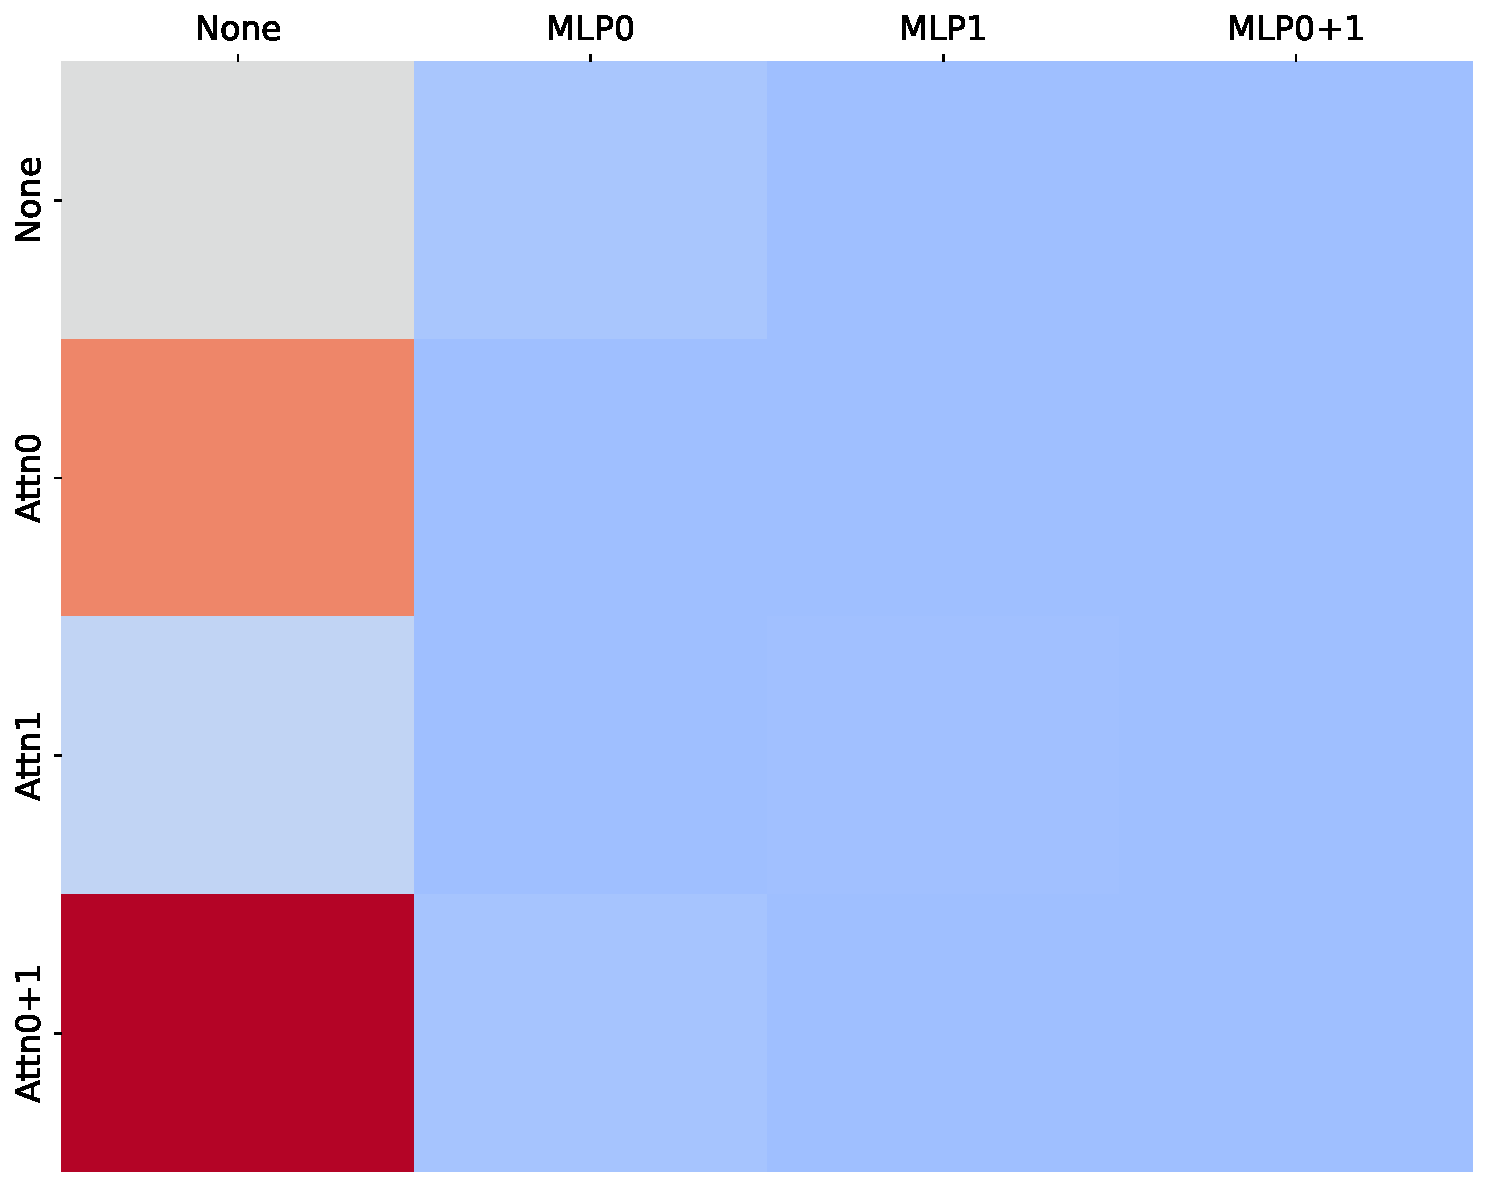
\includegraphics[width=\linewidth]{Figures/figures_circuit/interventions/bos_lower.pdf}
  \end{minipage}~
  % \hspace{-1em}
  \begin{minipage}{0.24\textwidth}
      \centering
      \subcaption{\small upper layers on \bos}
      \label{fig:appendix-ablation-bos-upper}
      \vspace{-.2em}
      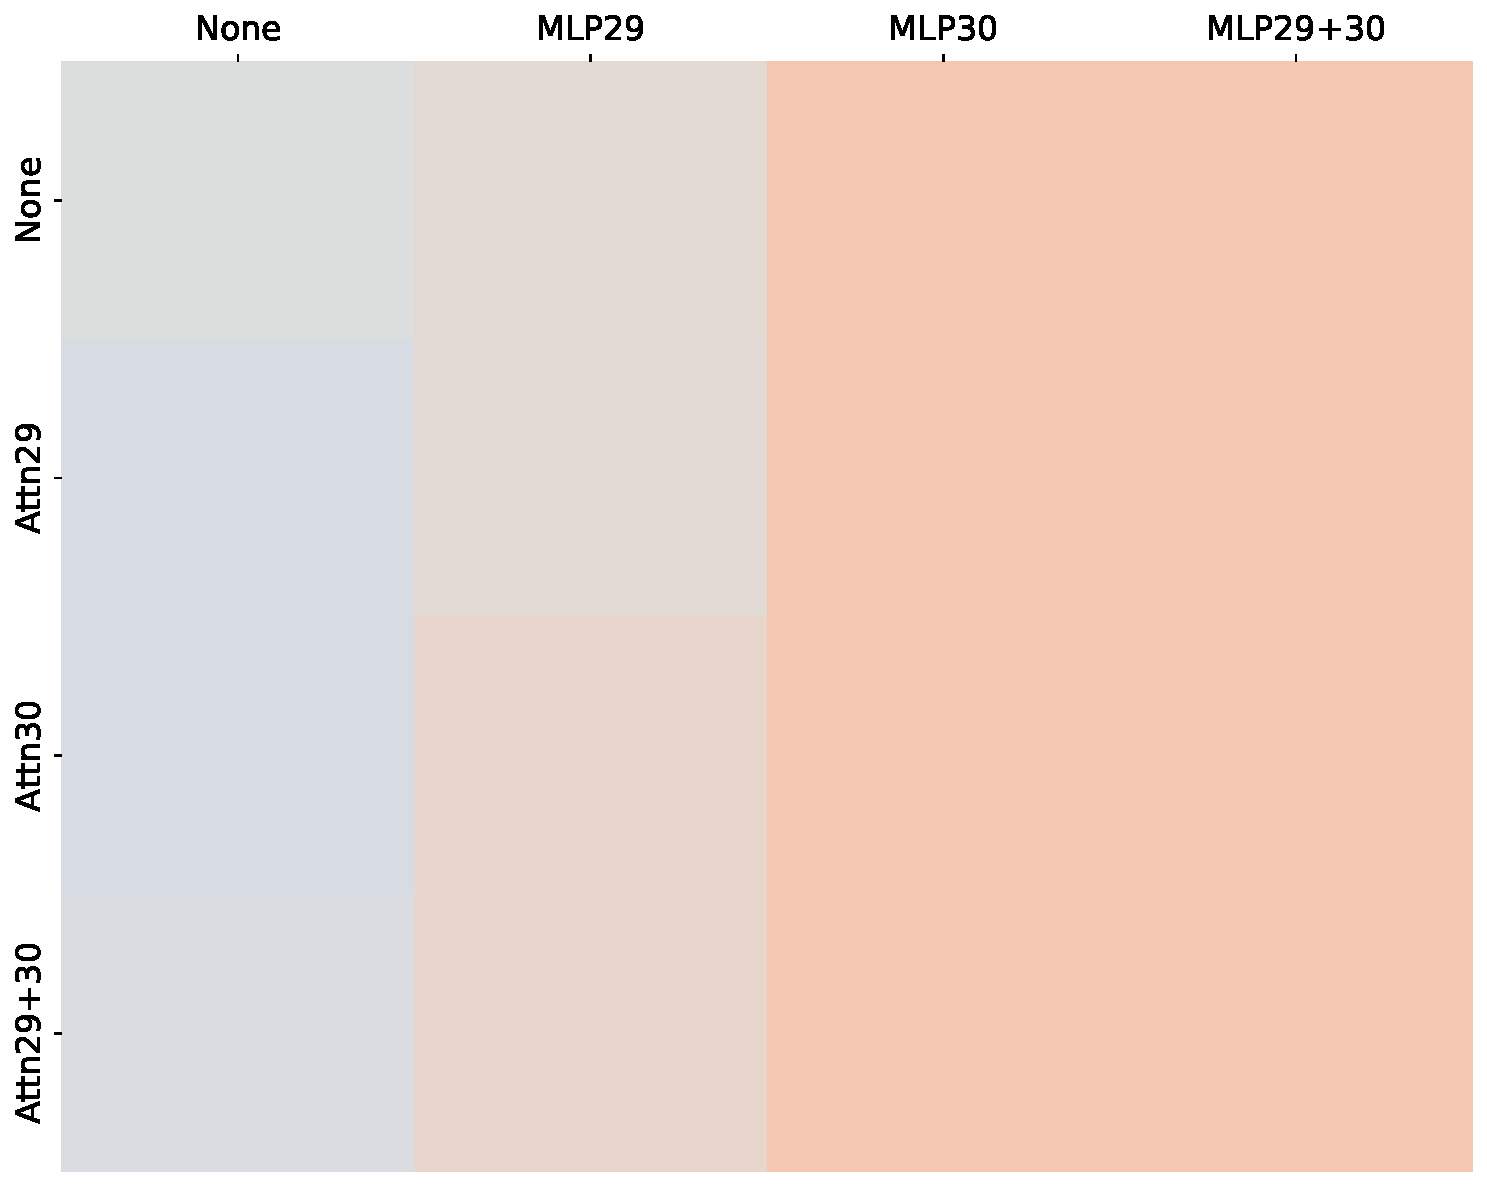
\includegraphics[width=\linewidth]{Figures/figures_circuit/interventions/bos_upper.pdf}
  \end{minipage}~
  % \hspace{-1em}
  \begin{minipage}{0.24\textwidth}
      \centering
      \subcaption{\small lower layers on \delim}
      \label{fig:appendix-ablation-delim-lower}
      \vspace{-.2em}
      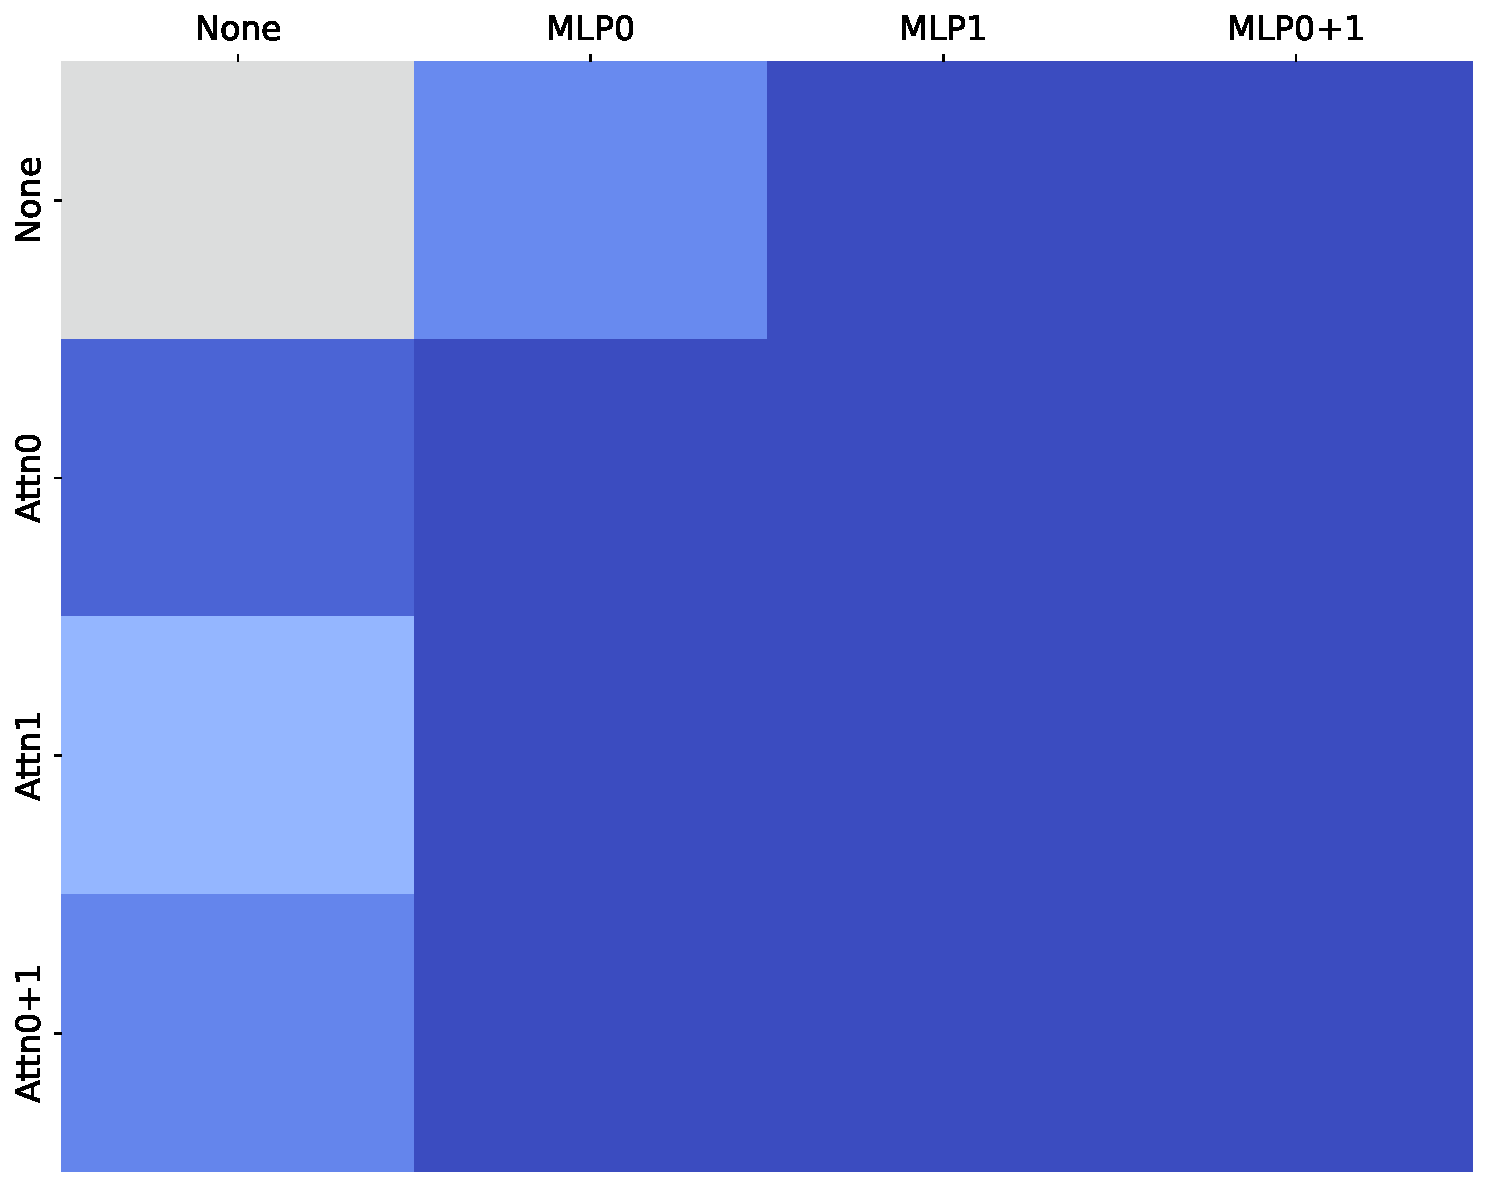
\includegraphics[width=\linewidth]{Figures/figures_circuit/interventions/delim_lower.pdf}
  \end{minipage}~
  % \vspace{-1em}
    \begin{minipage}{0.24\textwidth}
      \centering
      \subcaption{\small upper layers on \delim}
      \label{fig:appendix-ablation-delim-lower}
      \vspace{-.2em}
      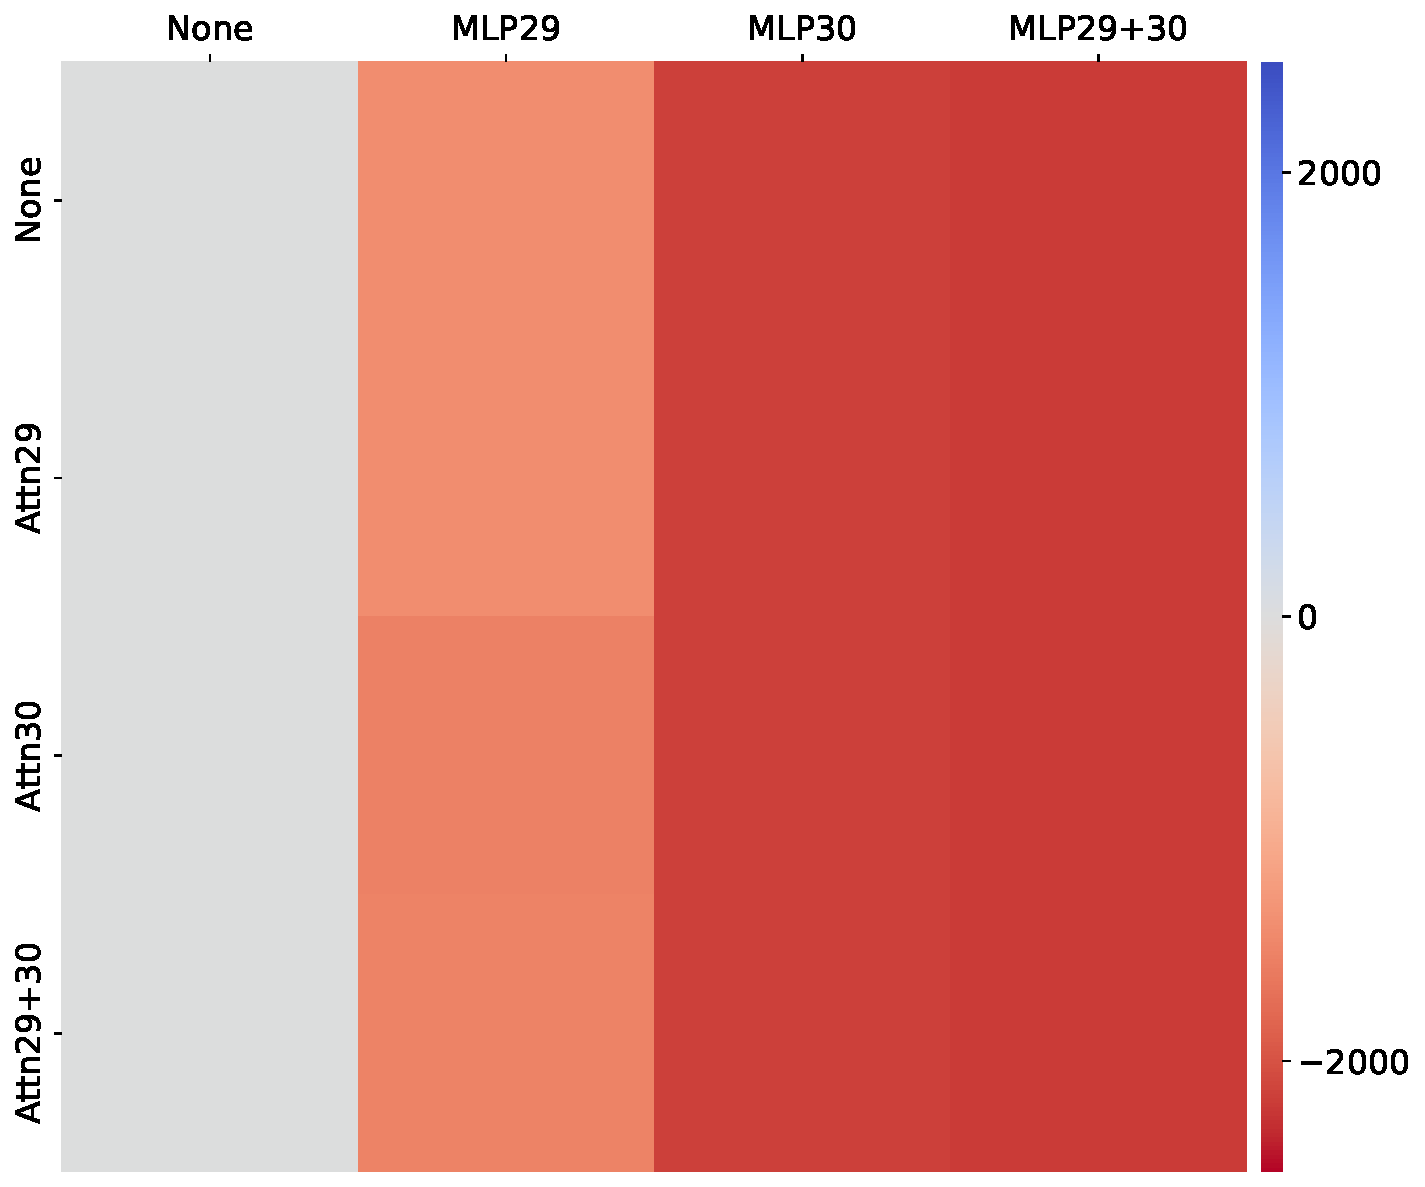
\includegraphics[width=\linewidth]{Figures/figures_circuit/interventions/delim_upper.pdf}
  \end{minipage}~
  
  \caption{\small The effect of $\MLP$ and $\Attn$ of lower and upper two layers on the norm of \bos and \delim.}
  \label{figure:appendix-ablation-massive-sup-control}
  % \vspace{-1em}
\end{figure}


\begin{figure}[t]
  \centering
  \begin{minipage}{0.33\textwidth}
      \centering
      \subcaption{\small Ablations on layer $0$}
      \label{fig:appendix-ablation-massive-sup-control-0}
      \vspace{-.2em}
      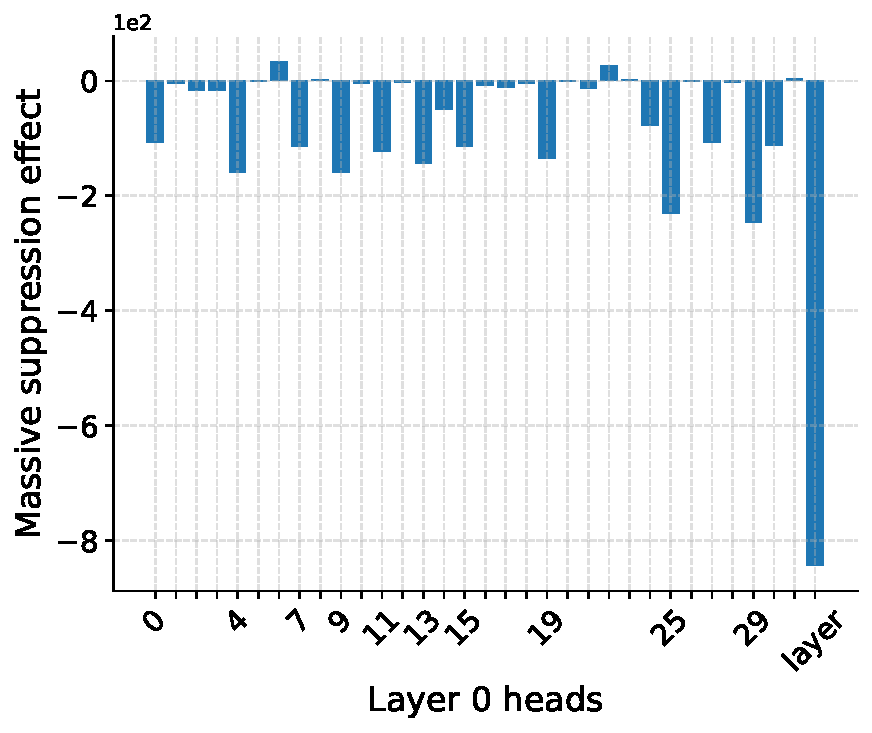
\includegraphics[width=\linewidth]{Figures/figures_circuit/interventions/bos_control/bos_massive_sup_L0.pdf}
  \end{minipage}~
  % \hspace{-1em}
  \begin{minipage}{0.33\textwidth}
      \centering
      \subcaption{\small Ablations on layer $1$}
      \label{fig:appendix-ablation-massive-sup-control-1}
      \vspace{-.2em}
      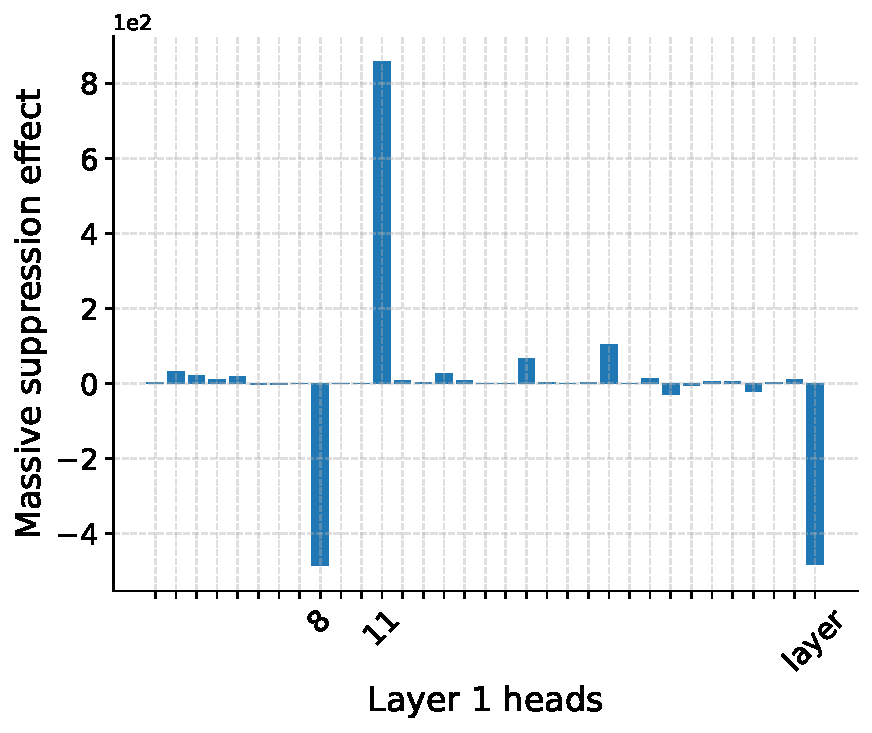
\includegraphics[width=\linewidth]{Figures/figures_circuit/interventions/bos_control/bos_massive_sup_L1.pdf}
  \end{minipage}~
  % \hspace{-1em}
  \begin{minipage}{0.33\textwidth}
      \centering
      \subcaption{\small Ablations on entire layer $0$}
      \label{fig:appendix-ablation-massive-sup-control-attn}
      \vspace{-.2em}
      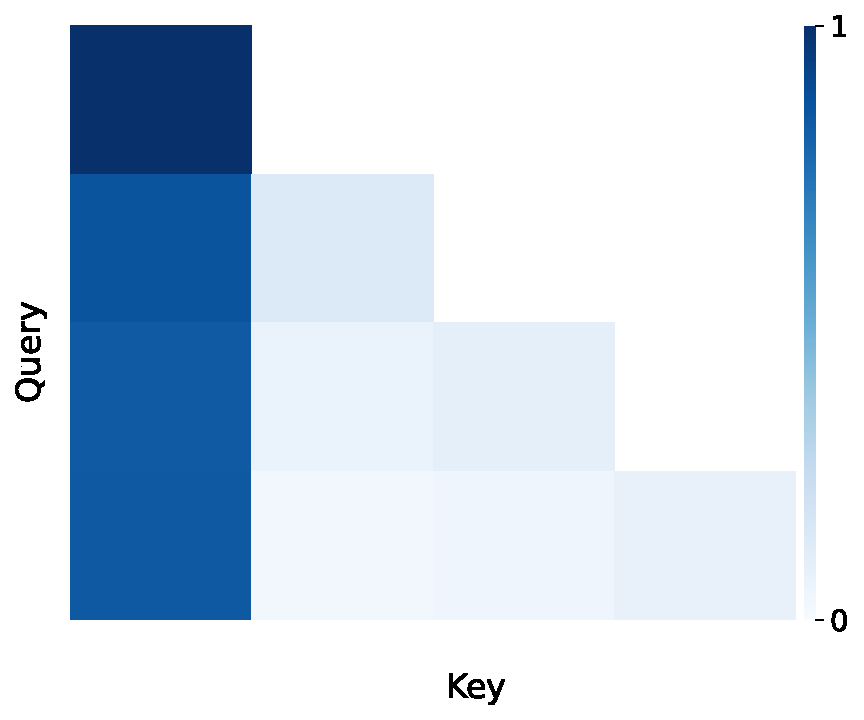
\includegraphics[width=\linewidth]{Figures/figures_circuit/interventions/bos_control/L0_intervention_attn_weights.pdf}
  \end{minipage}~
  % \vspace{-1em}
  
  \caption{\small Ablations using control sample
  }
  \label{figure:appendix-ablation-massive-sup-control}
  % \vspace{-1em}
\end{figure}

\begin{figure}[t]
  \centering
  \begin{minipage}{0.33\textwidth}
      \centering
      \subcaption{\small Ablations on layer $0$}
      \label{fig:appendix-ablation-massive-sup-zero-0}
      \vspace{-.2em}
      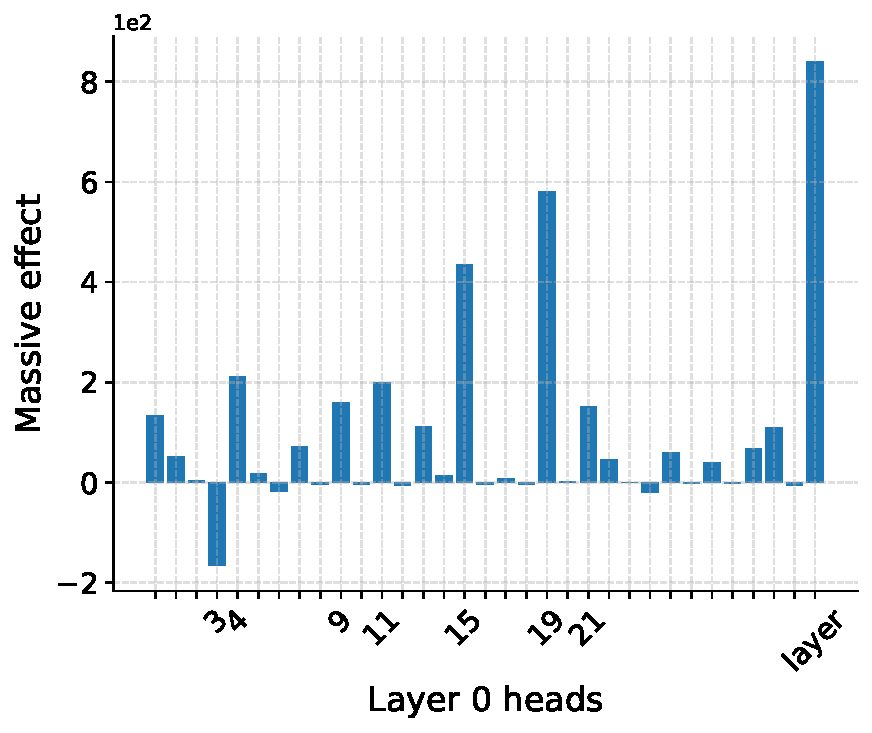
\includegraphics[width=\linewidth]{Figures/figures_circuit/interventions/bos_zero_out/bos_massive_L0.pdf}
  \end{minipage}~
  % \hspace{-1em}
  \begin{minipage}{0.33\textwidth}
      \centering
      \subcaption{\small Ablations on layer $1$}
      \label{fig:appendix-ablation-massive-sup-zero-1}
      \vspace{-.2em}
      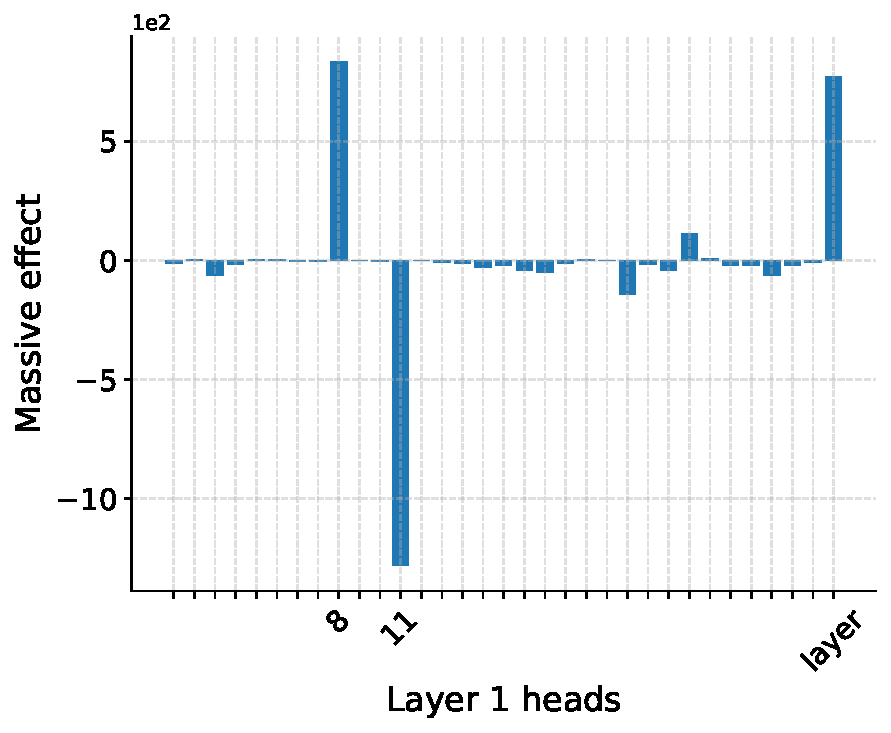
\includegraphics[width=\linewidth]{Figures/figures_circuit/interventions/bos_zero_out/bos_massive_L1.pdf}
  \end{minipage}~
  % \hspace{-1em}
  \begin{minipage}{0.33\textwidth}
      \centering
      \subcaption{\small Ablations on entire layer $0$}
      \label{fig:appendix-ablation-massive-sup-zero-attn}
      \vspace{-.2em}
      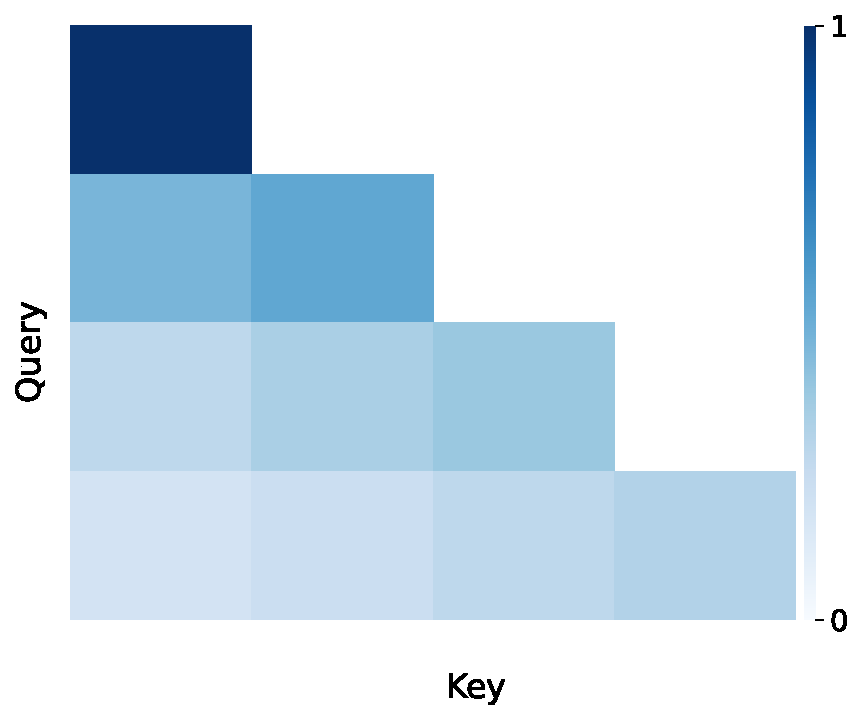
\includegraphics[width=\linewidth]{Figures/figures_circuit/interventions/bos_zero_out/L0_zero_attn_weights.pdf}
  \end{minipage}~
  % \vspace{-1em}
  
  \caption{\small Ablations using zeroing-out
  }
  \label{figure:appendix-ablation-massive-zero}
  % \vspace{-1em}
\end{figure}

\begin{figure}[t]
  \centering
  \begin{minipage}{0.33\textwidth}
      \centering
      \subcaption{\small Ablations on layer $0$}
      \label{fig:appendix-ablation-delim-0}
      \vspace{-.2em}
      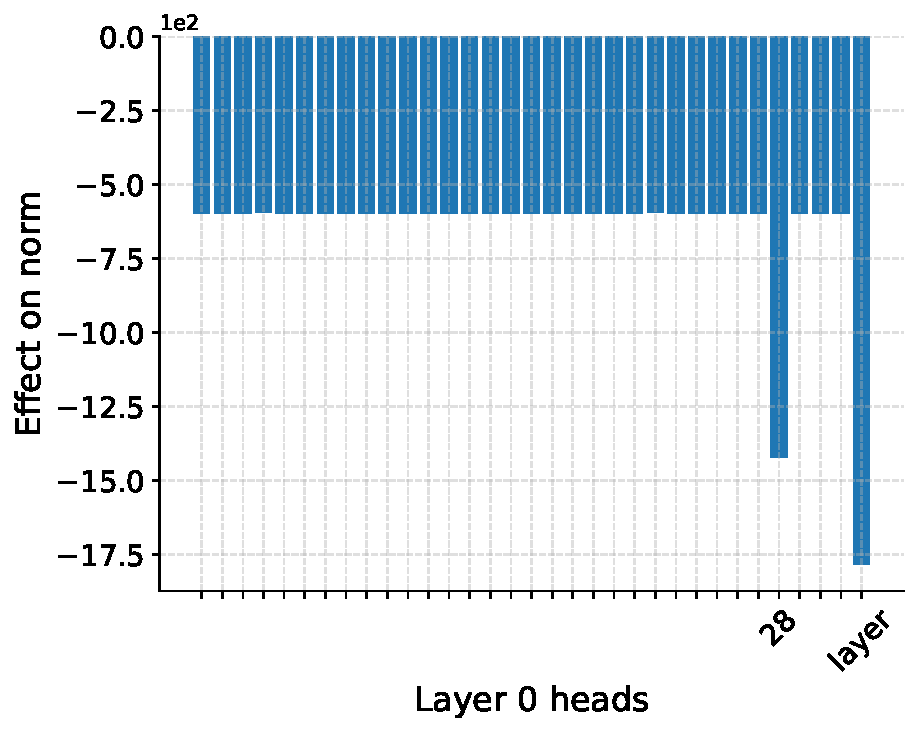
\includegraphics[width=\linewidth]{Figures/figures_circuit/interventions/delim_no_rope/delim_massive_suppression_L0.pdf}
  \end{minipage}~
  % \hspace{-1em}
  \begin{minipage}{0.33\textwidth}
      \centering
      \subcaption{\small Ablations on layer $1$}
      \label{fig:appendix-ablation-delim-1}
      \vspace{-.2em}
      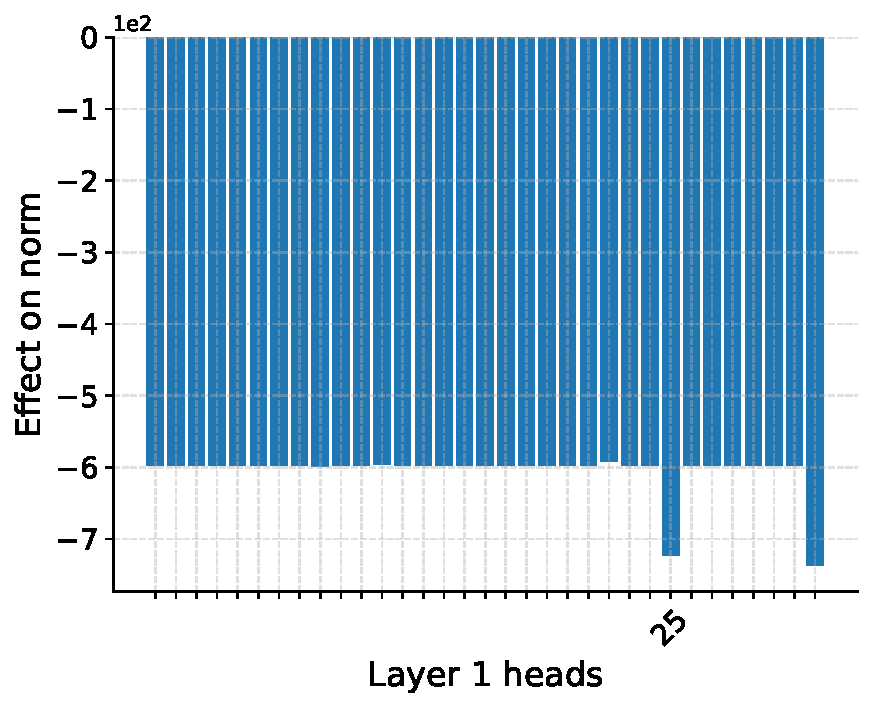
\includegraphics[width=\linewidth]{Figures/figures_circuit/interventions/delim_no_rope/delim_massive_suppression_L1.pdf}
  \end{minipage}~
  % \hspace{-1em}
  \begin{minipage}{0.33\textwidth}
      \centering
      \subcaption{\small Ablations on entire layer $0$}
      \label{fig:appendix-ablation-delim-attn}
      \vspace{-.2em}
      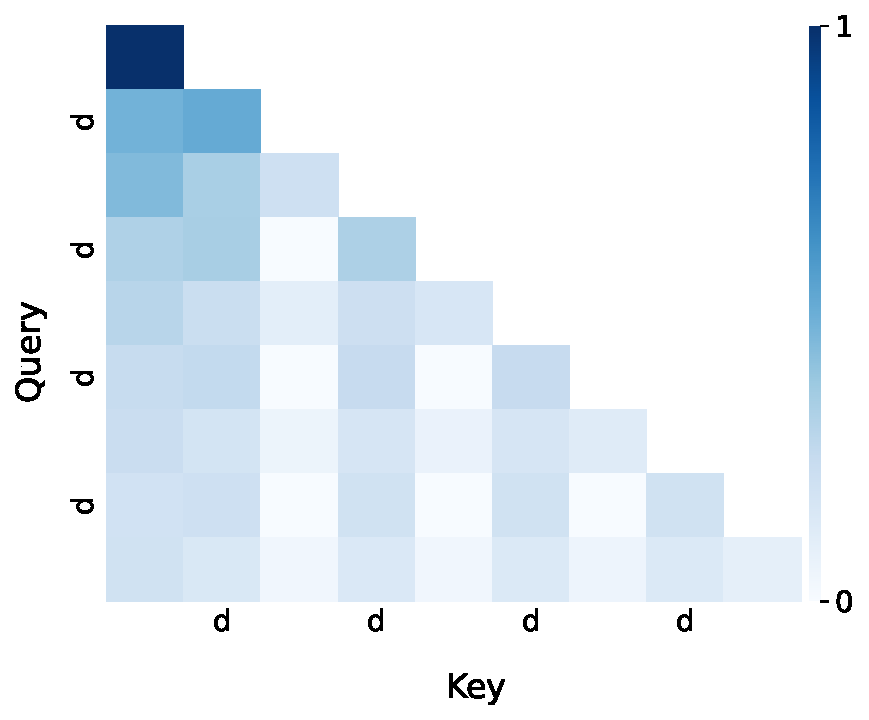
\includegraphics[width=\linewidth]{Figures/figures_circuit/interventions/delim_no_rope/L0_no_rope_attn_weights.pdf}
  \end{minipage}~
  % \vspace{-1em}
  
  \caption{\small Ablations using no \rope
  }
  \label{figure:appendix-ablation-delim}
  % \vspace{-1em}
\end{figure}


\subsection{Supporting Results for \Cref{sub:lots_of_dormant_heads}} \label{sub:app_supporting_lots_of_heads}


\begin{figure}
    \centering
    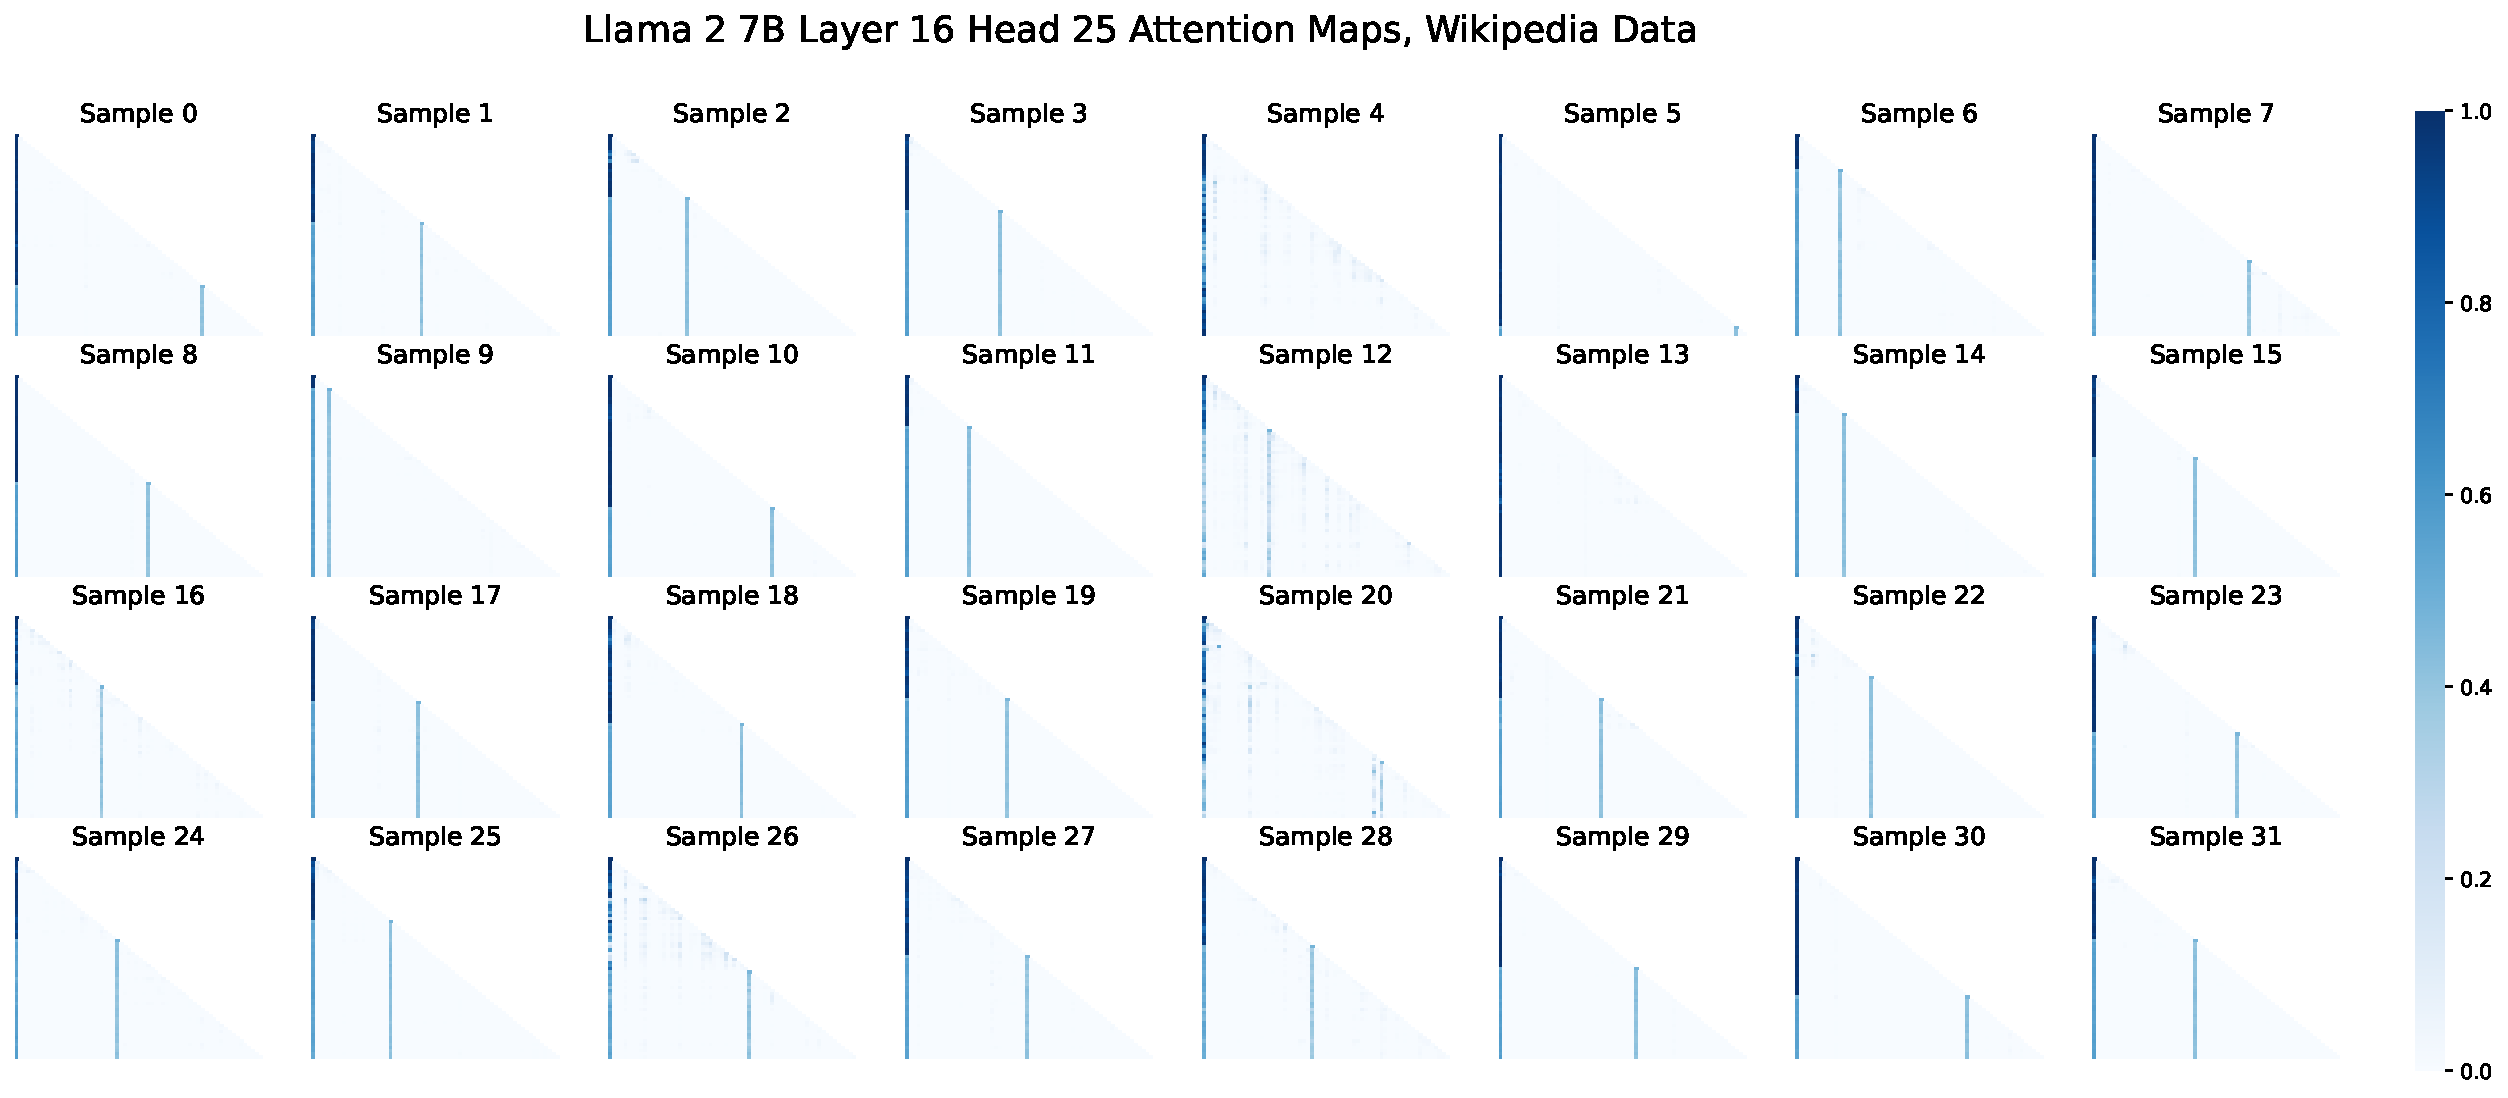
\includegraphics[width=\textwidth]{Figures/L16_H25/attn_maps_l16h25_wiki.pdf}
    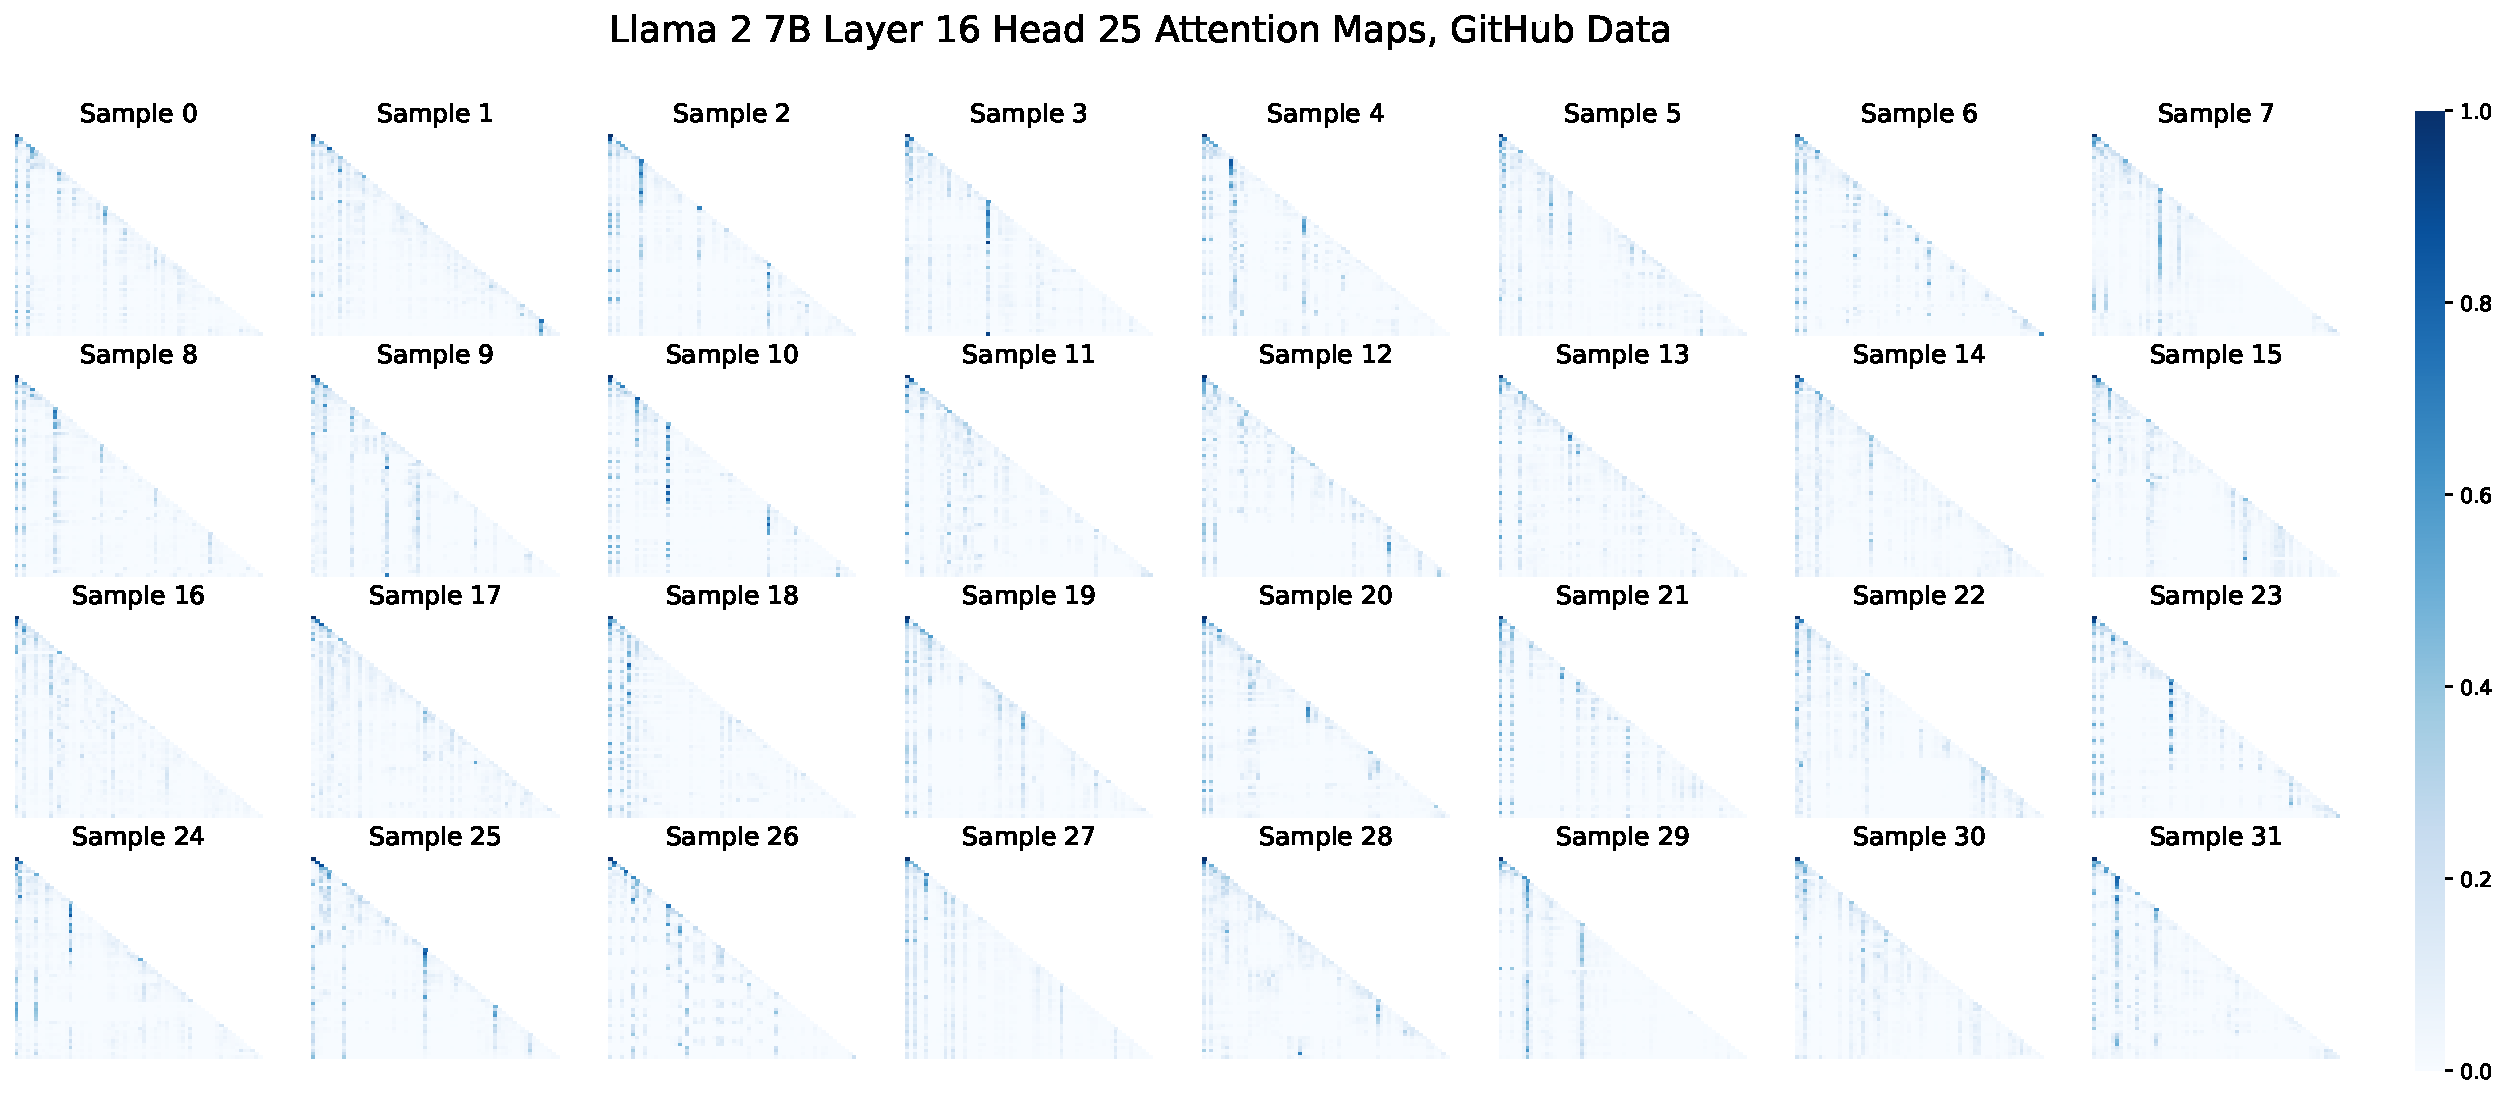
\includegraphics[width=\textwidth]{Figures/L16_H25/attn_maps_l16h25_github.pdf}
    \caption{\small\textbf{Visualizations of attention weights for Llama 2 7B Layer 16 Head 25 on both Wikipedia and GitHub data.} A continuation of \Cref{fig:attn_l16_h25_small}.}
    \label{fig:attn_l16_h25_improved}
\end{figure}

\begin{figure}
    \centering
    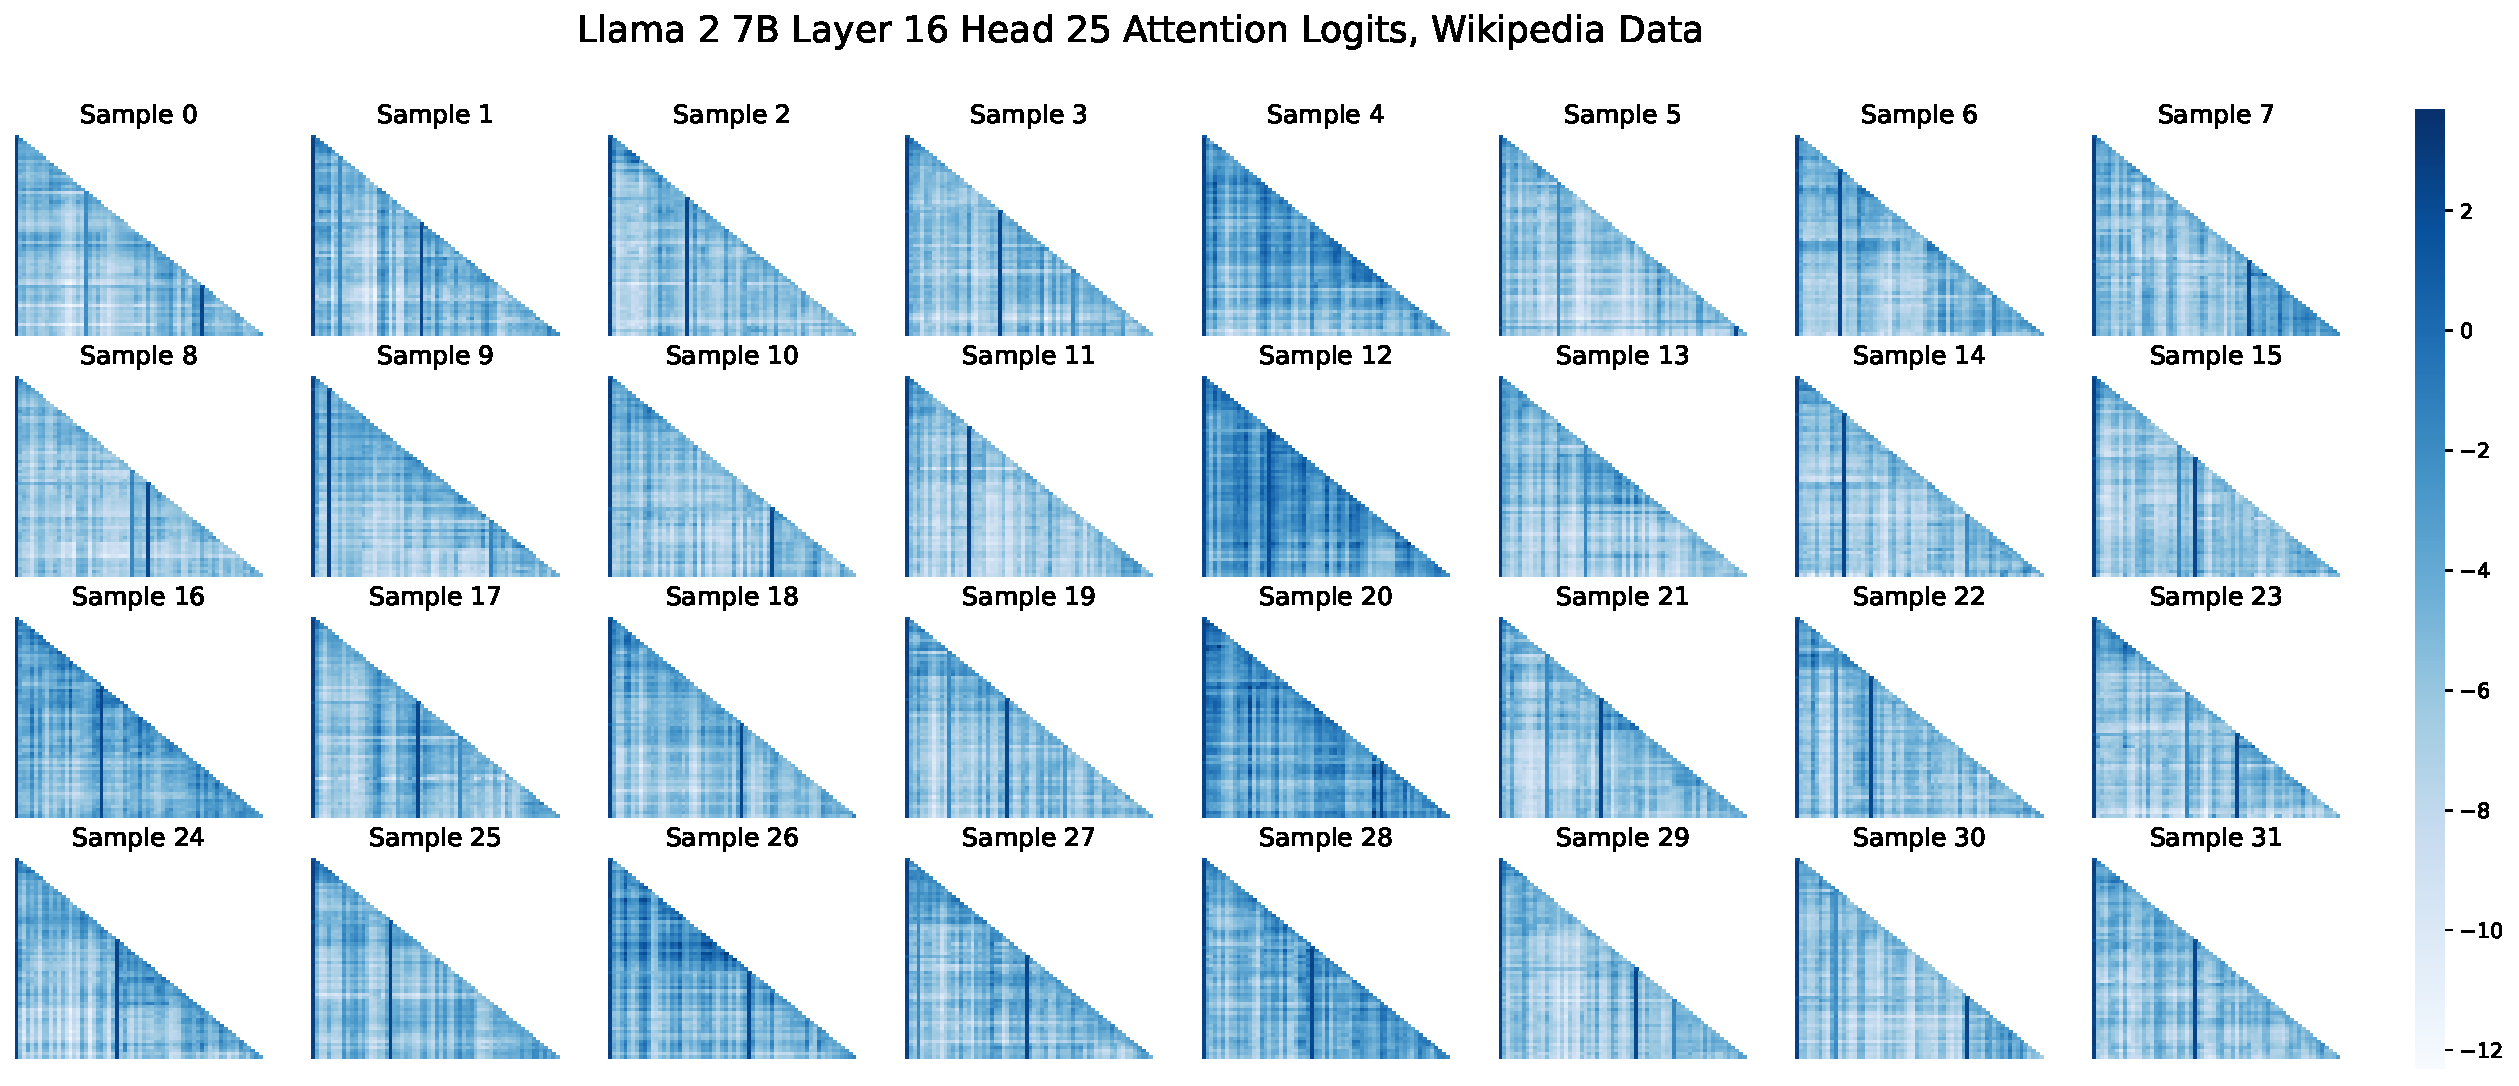
\includegraphics[width=\textwidth]{Figures/L16_H25/attn_logits_l16h25_wiki.pdf}
    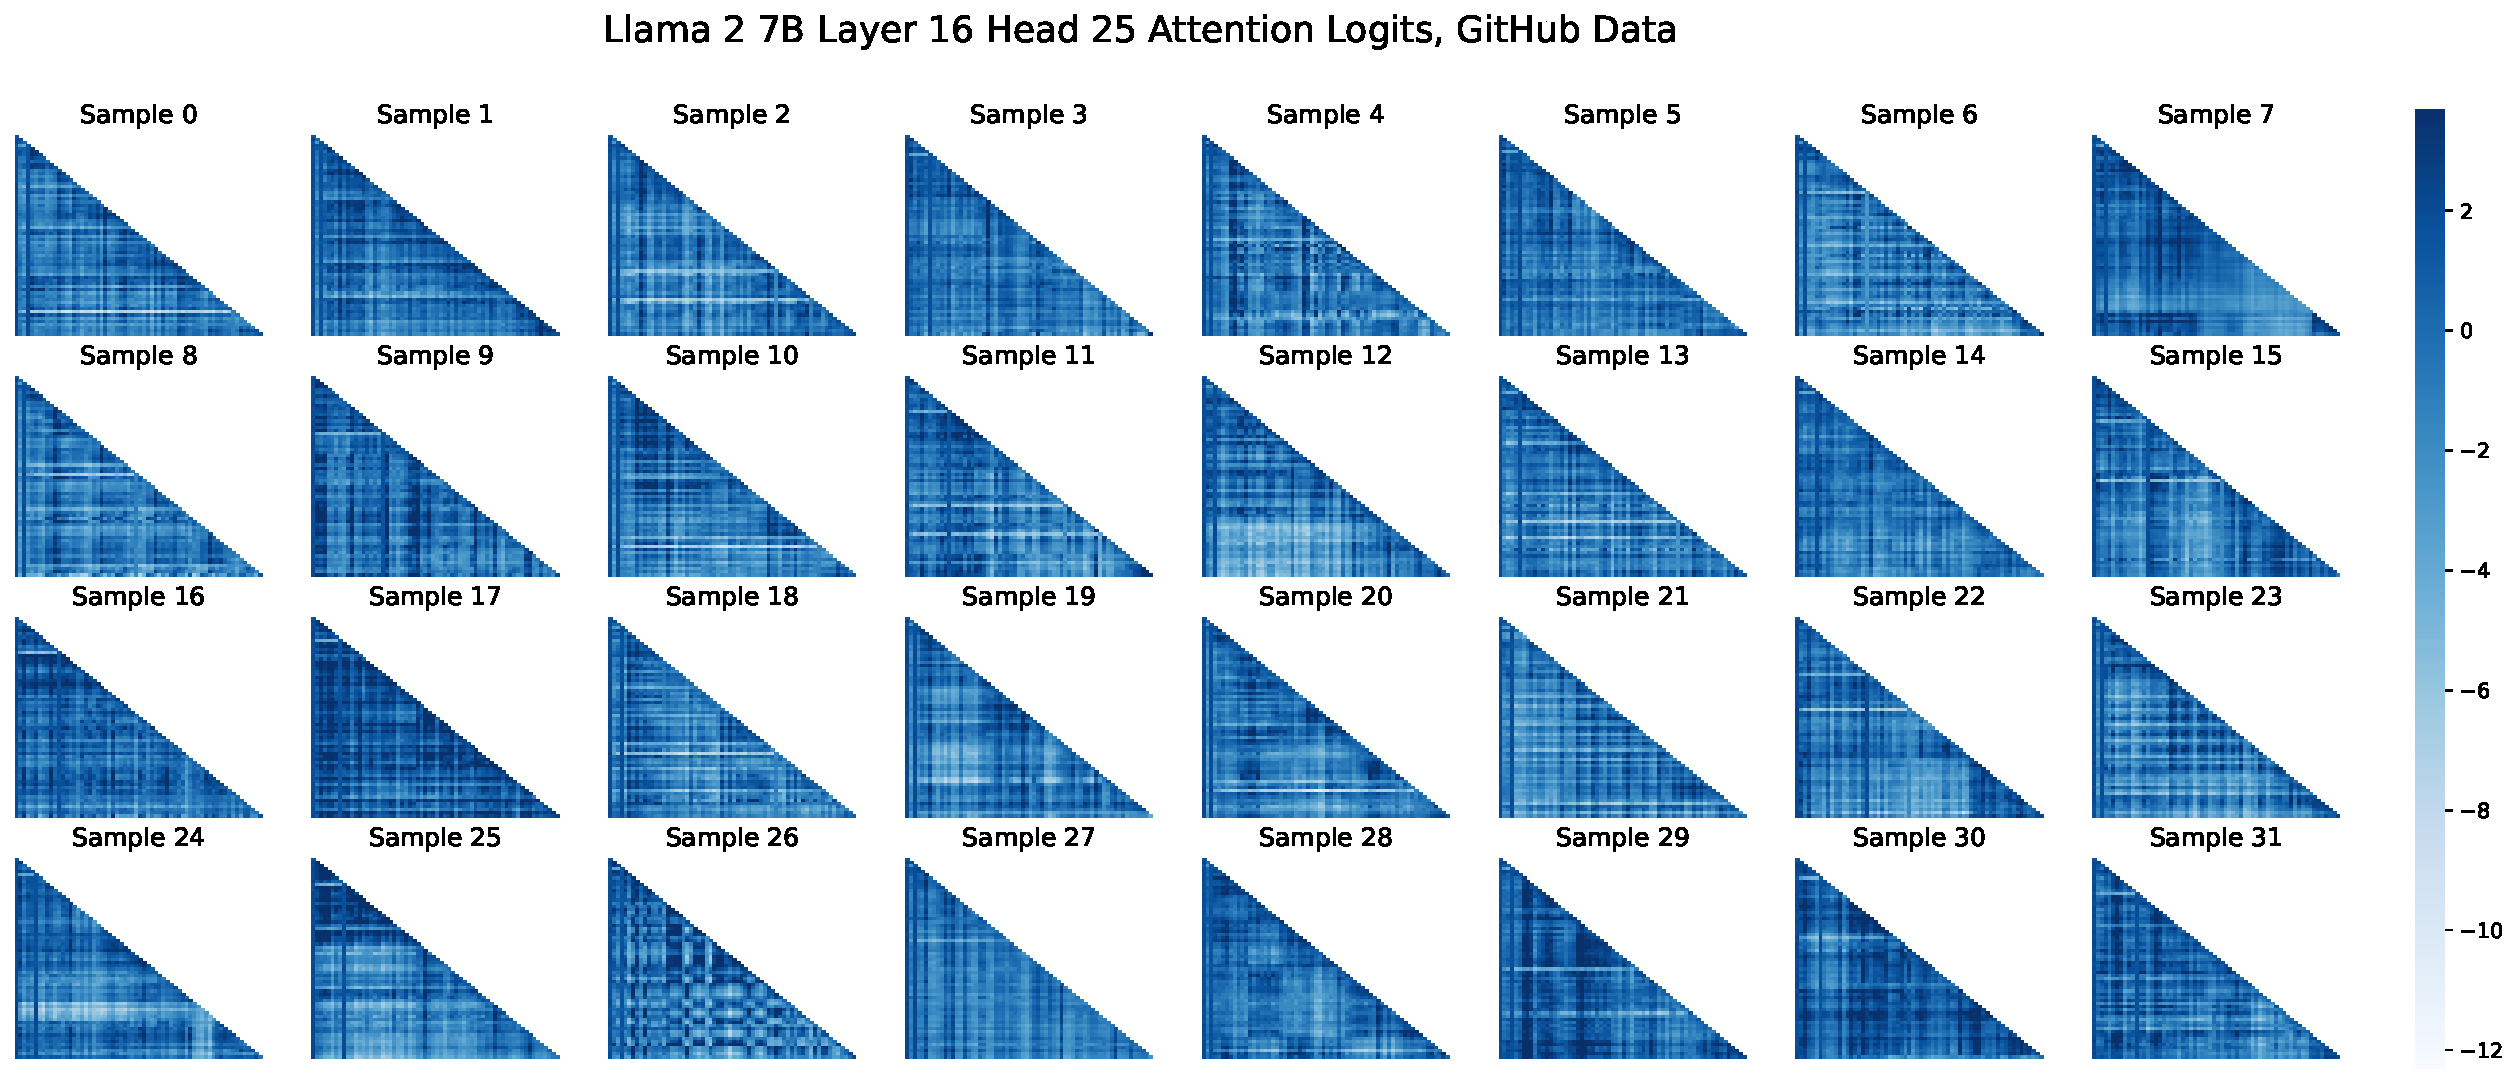
\includegraphics[width=\textwidth]{Figures/L16_H25/attn_logits_l16h25_github.pdf}
    \caption{\small\textbf{Visualizations of pre-softmax attention logits for Llama 2 7B Layer 16 Head 25 on both Wikipedia and GitHub data.} A continuation of \Cref{fig:attn_logits_l16_h25_small}.}
    \label{fig:attn_logits_l16_h25_improved}
\end{figure}

\subsection{Supporting Results for \Cref{sub:controlled_experiments}} \label{sub:app_supporting_controlled}

\subsection{Task in \citet{bietti2024birth}}
\begin{figure}[t]
  \centering
  \begin{minipage}{0.4\textwidth}
      \centering
      \subcaption{\small Data generating procedure}
      \label{fig:appendix-pretraining-dgp}
      \vspace{-.2em}
      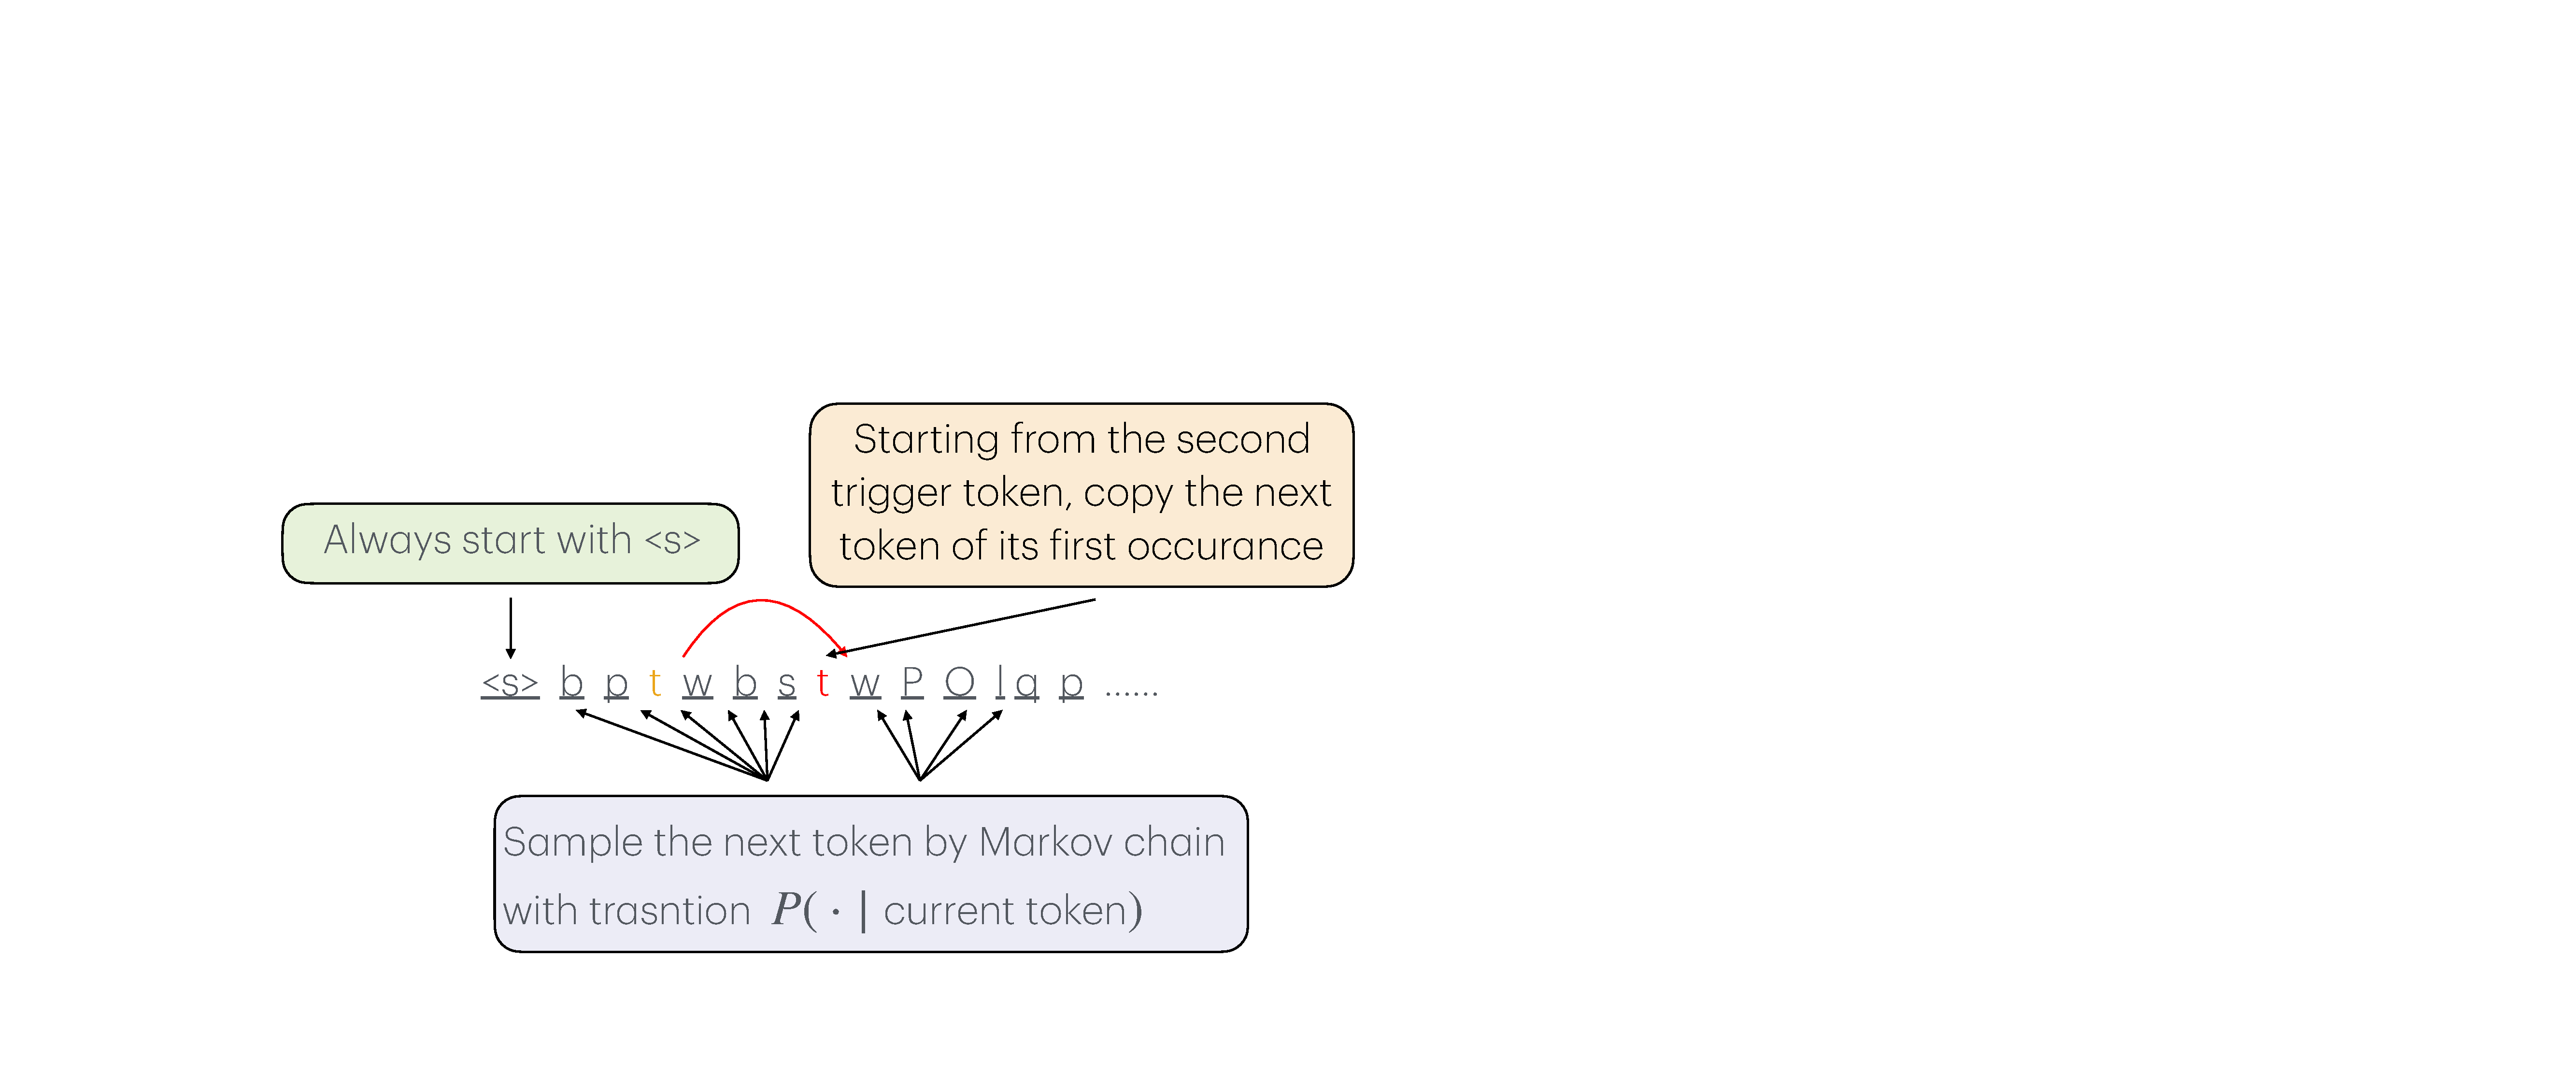
\includegraphics[width=\linewidth]{Figures/figures_pretraining/Biette.pdf}
  \end{minipage}
  \hspace{-1em}
  \begin{minipage}{0.3\textwidth}
      \centering
      \subcaption{\small Layer 0 on dormant sequence}
      \label{fig:appendix-biette-attn-weights-dormant-l0}
      \vspace{-.2em}
      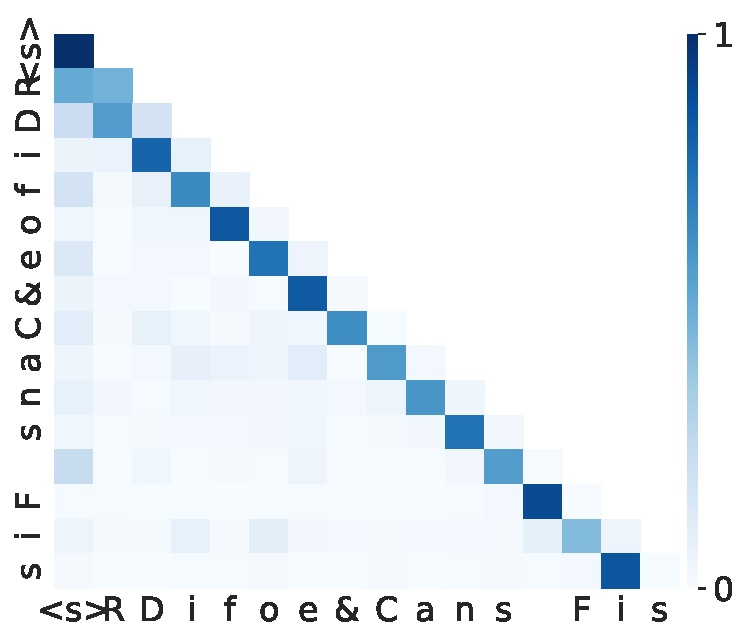
\includegraphics[width=\linewidth]{Figures/figures_pretraining/Biette_attn_weights_seq0_layer0.pdf}
  \end{minipage}
  \hspace{-1em}
    \begin{minipage}{0.3\textwidth}
      \centering
      \subcaption{\small Layer 1 on dormant sequence}
      \label{fig:appendix-biette-attn-weights-dormant-l1}
      \vspace{-.2em}
      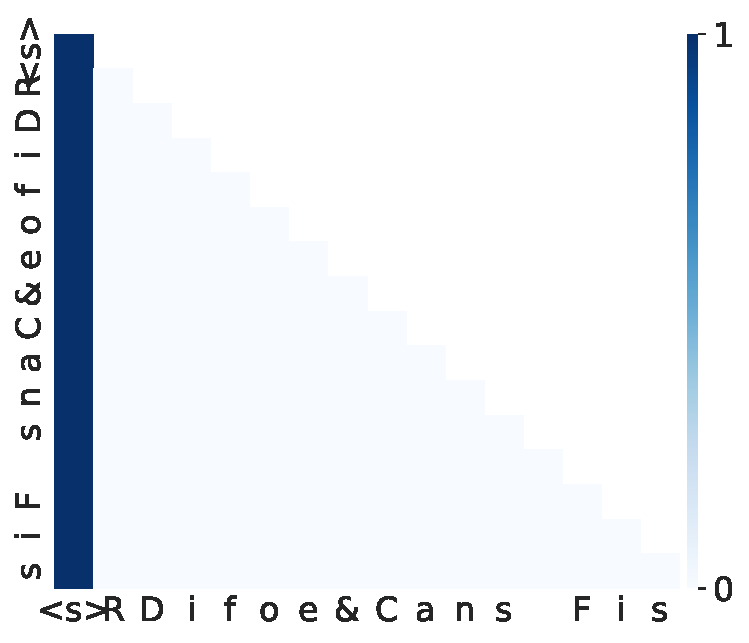
\includegraphics[width=\linewidth]{Figures/figures_pretraining/Biette_attn_weights_seq0_layer1.pdf}
  \end{minipage}
  \vspace{-1em}
  \caption{\small Using the task in \citet{bietti2024birth}}
  \label{figure:appendix-pretraining-biette-findings}
  \vspace{-1em}
\end{figure}

\begin{figure}
\centering
  \begin{minipage}{0.45\textwidth}
      \centering
      \subcaption{\small Layer 0 on active sequence}
      \label{fig:appendix-biette-attn-weights-active-l0}
      \vspace{-.2em}
      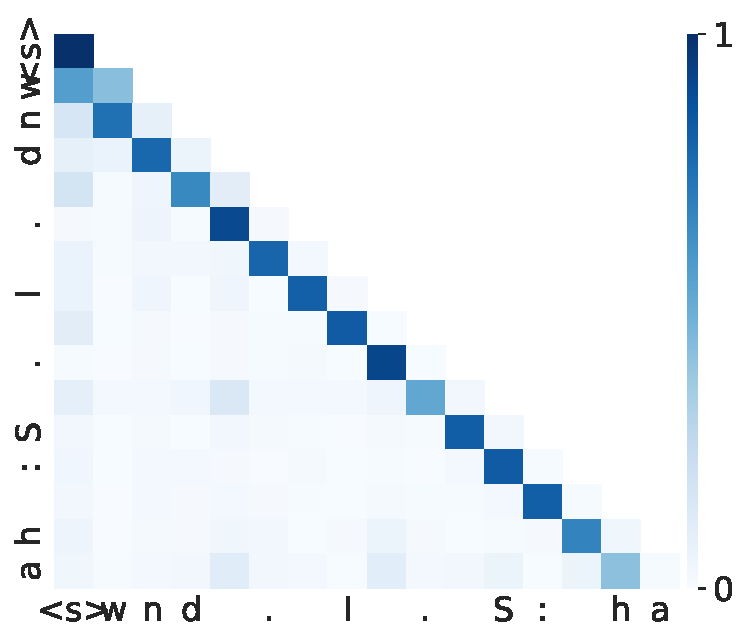
\includegraphics[width=\linewidth]{Figures/figures_pretraining/Biette_attn_weights_seq1_layer0.pdf}
  \end{minipage}
  \hspace{-1em}
    \begin{minipage}{0.45\textwidth}
      \centering
      \subcaption{\small Layer 1 on active sequence}
      \label{fig:appendix-biette-attn-weights-active-l1}
      \vspace{-.2em}
      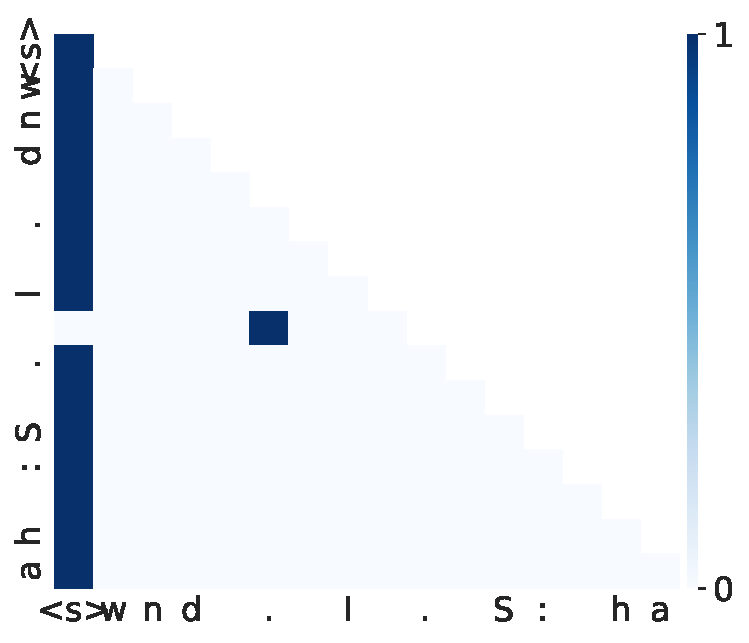
\includegraphics[width=\linewidth]{Figures/figures_pretraining/Biette_attn_weights_seq1_layer1.pdf}
  \end{minipage}
  \vspace{-1em}
  \caption{\small Using the task in \citet{bietti2024birth}}
  \label{figure:appendix-pretraining-biette-findings-1}
  \vspace{-1em}
\end{figure}

\begin{figure}
      \centering
  \begin{minipage}{0.45\textwidth}
      \centering
      \subcaption{\small Output norm on layer 1}
      \label{fig:appendix-biette-massive}
      \vspace{-.2em}
      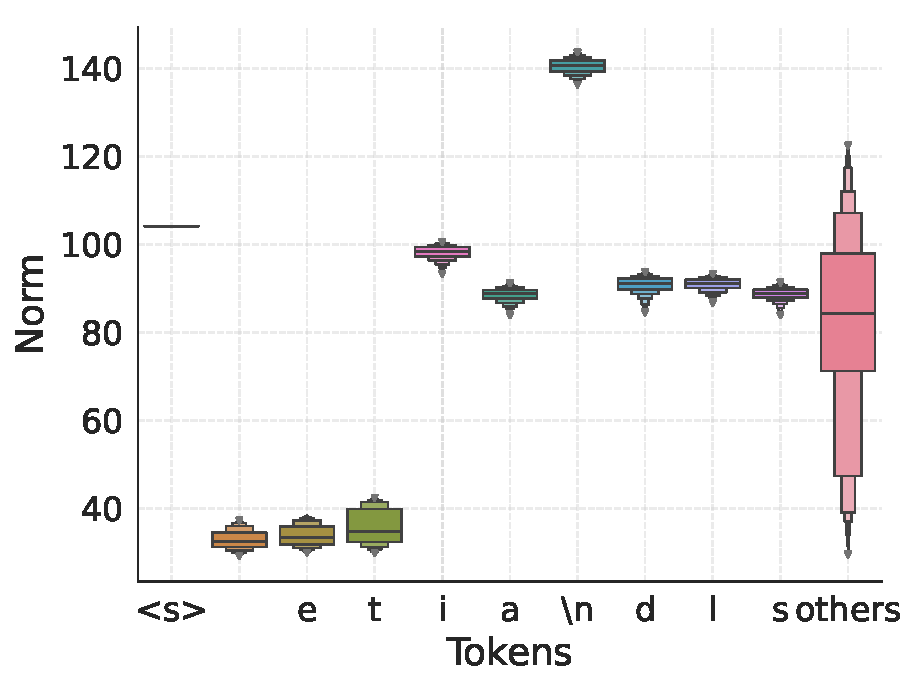
\includegraphics[width=\linewidth]{Figures/figures_pretraining/Biette/Biette_L3_massive.pdf}
  \end{minipage}
  \hspace{-1em}
    \begin{minipage}{0.45\textwidth}
      \centering
      \subcaption{\small Value state norm on layer 2}
      \label{fig:appendix-biette-minor}
      \vspace{-.2em}
      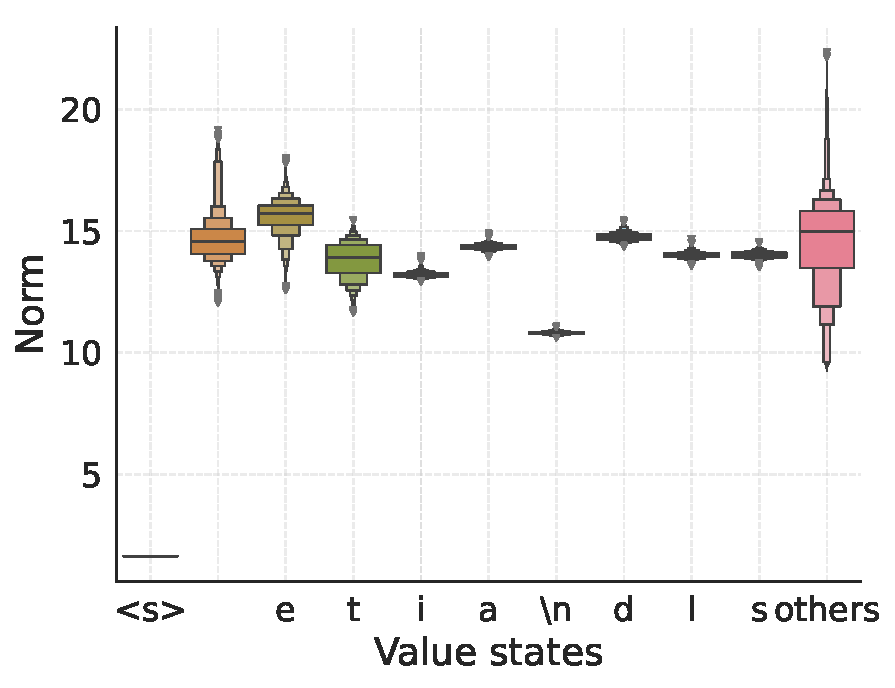
\includegraphics[width=\linewidth]{Figures/figures_pretraining/Biette/Biette_L3_minor.pdf}
  \end{minipage}
  \vspace{-1em}
  \caption{\small Using the task in \citet{bietti2024birth}}
  \label{figure:appendix-pretraining-biette-findings-3}
  \vspace{-1em}
\end{figure}

\subsection{The ``dormant Markov task''}
\begin{figure}[t]
  \centering
  \begin{minipage}{0.4\textwidth}
      \centering
      \subcaption{\small Data generating procedure}
      \label{fig:appendix-pretraining-dgp-dormant-markov}
      \vspace{-.2em}
      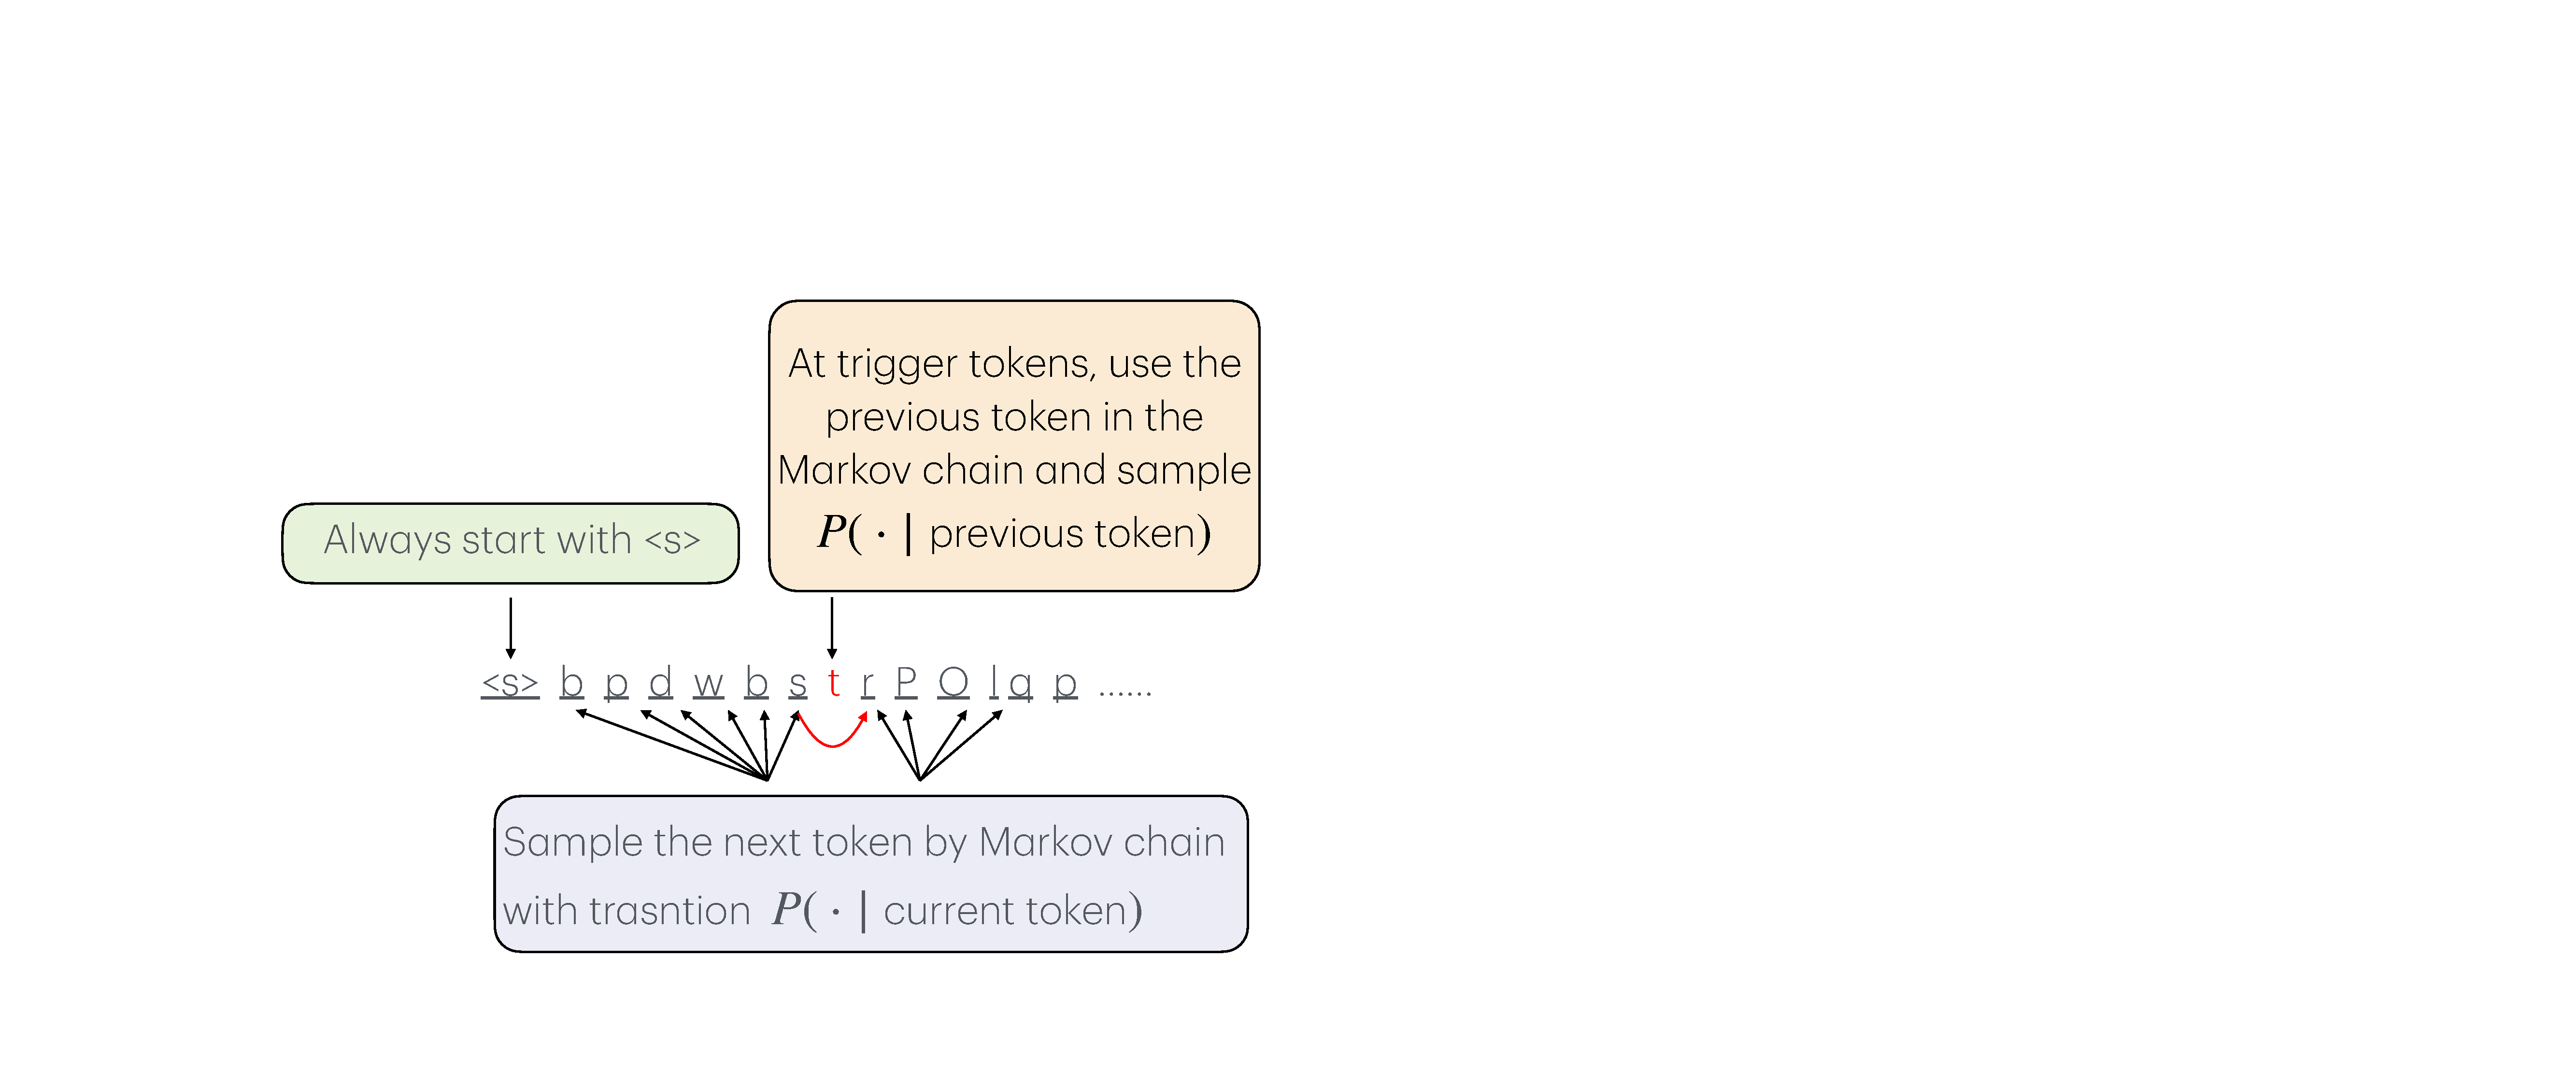
\includegraphics[width=\linewidth]{Figures/figures_pretraining/dormant_markov.pdf}
  \end{minipage}
  \hspace{-1em}
  \begin{minipage}{0.3\textwidth}
      \centering
      \subcaption{\small Layer 0 on dormant sequence}
      \label{fig:appendix-dormant-markov-attn-weights-dormant}
      \vspace{-.2em}
      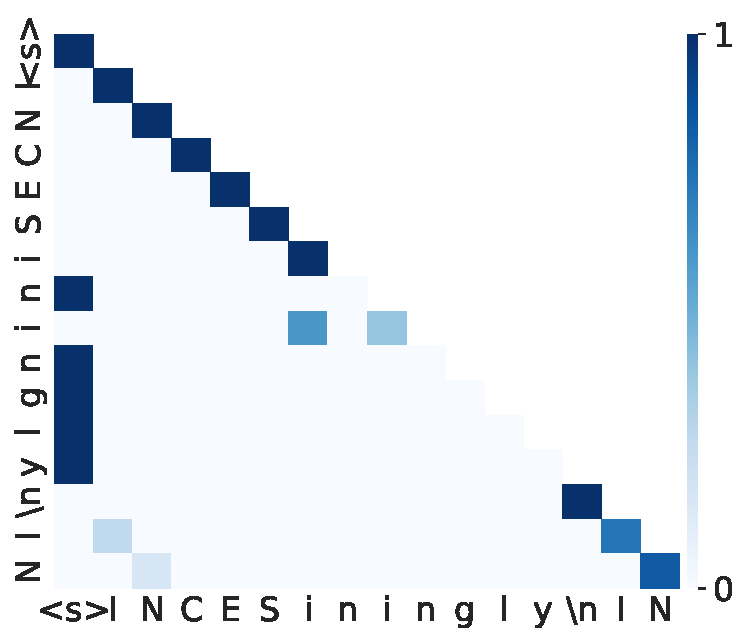
\includegraphics[width=\linewidth]{Figures/figures_pretraining/dormant_markov/dormant_markov_attn_weights_seq0.pdf}
  \end{minipage}
  \hspace{-1em}
  \begin{minipage}{0.3\textwidth}
      \centering
      \subcaption{\small Layer 0 on active sequence}
      \label{fig:appendix-dormant-markov-attn-weights-active}
      \vspace{-.2em}
      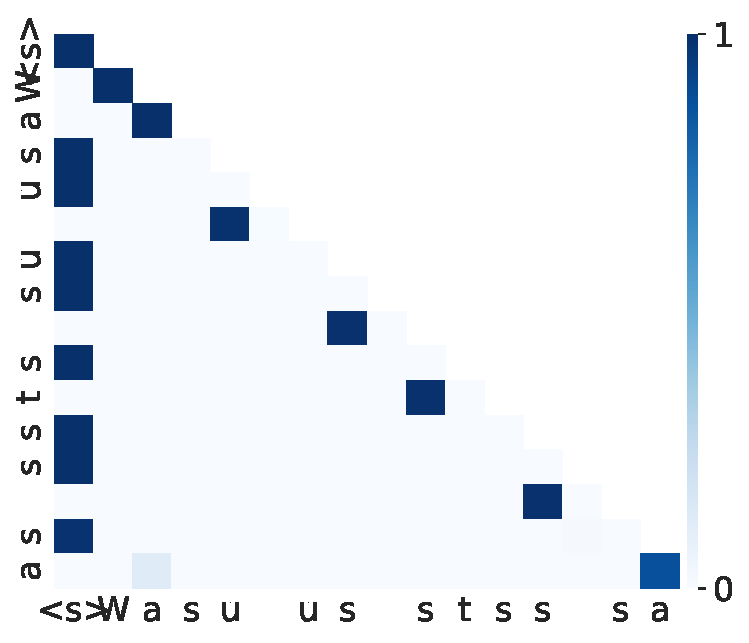
\includegraphics[width=\linewidth]{Figures/figures_pretraining/dormant_markov/dormant_markov_attn_weights_seq1.pdf}
  \end{minipage}
  \vspace{-1em}
  \caption{\small Dormant markov task}
  \label{figure:appendix-pretraining-dormant-markov-1}
  \vspace{-1em}
\end{figure}

\begin{figure}
      \centering
  \begin{minipage}{0.45\textwidth}
      \centering
      \subcaption{\small Output norm on layer 1}
      \label{fig:appendix-dormant-markov-massive}
      \vspace{-.2em}
      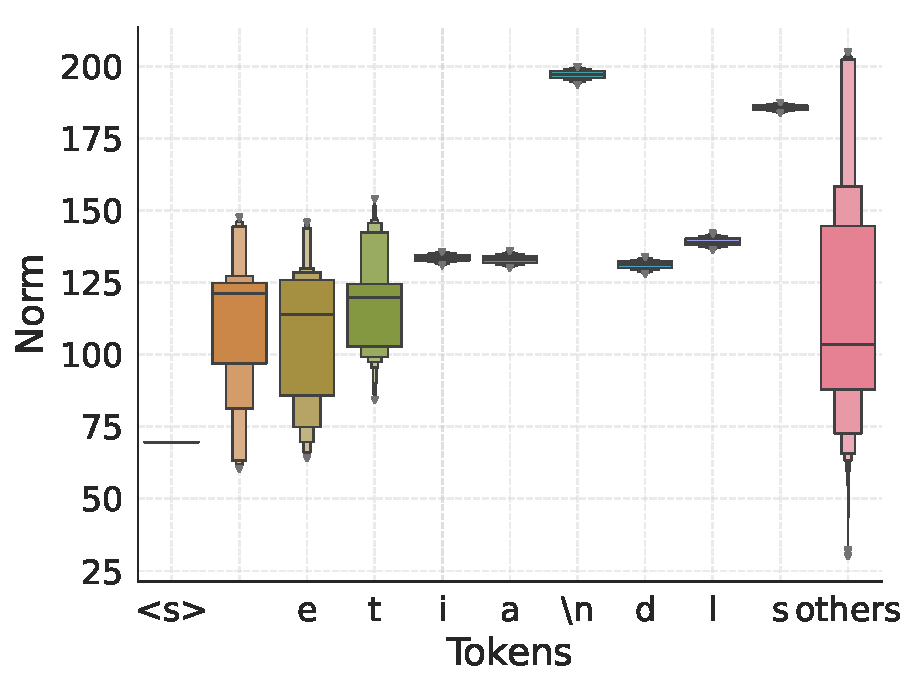
\includegraphics[width=\linewidth]{Figures/figures_pretraining/dormant_markov/dormant_markov_L3_massive.pdf}
  \end{minipage}
  \hspace{-1em}
    \begin{minipage}{0.45\textwidth}
      \centering
      \subcaption{\small Value state norm on layer 2}
      \label{fig:appendix-dormant-markov-minor}
      \vspace{-.2em}
      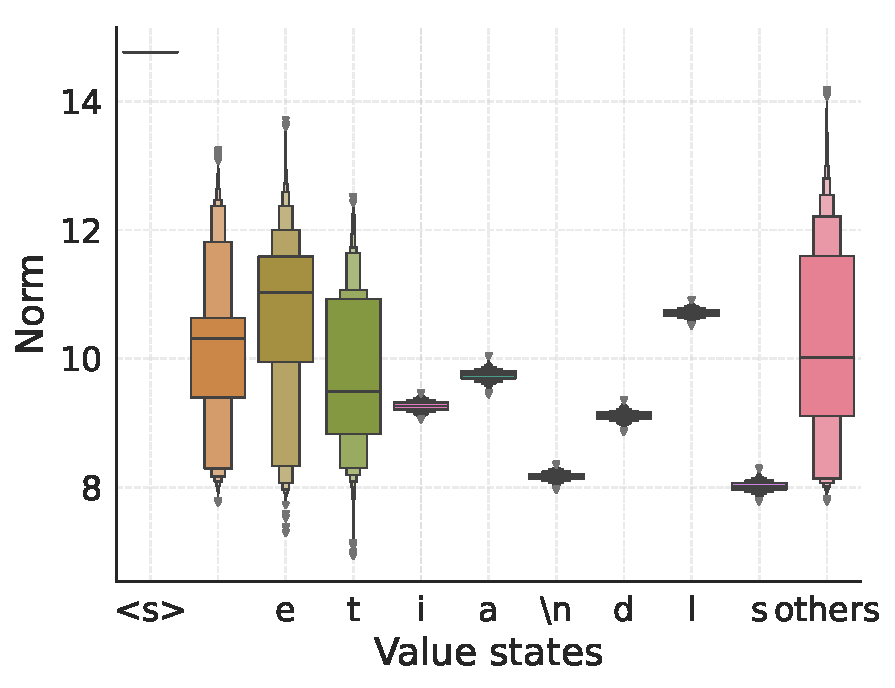
\includegraphics[width=\linewidth]{Figures/figures_pretraining/dormant_markov/dormant_markov_L3_minor.pdf}
  \end{minipage}
  \vspace{-1em}
  \caption{\small Dormant markov task}
  \label{figure:appendix-pretraining-dormant-markov-findings-2}
  \vspace{-1em}
\end{figure}